\chapter{（可选）扩散模型与最优传输}\label{ch:ot-eot}



将一个分布映射到另一个分布（生成是其特例）是一个核心挑战。流匹配通过学习一个随时间变化的速度场来应对此问题，该速度场将质量从源分布传输到目标分布。这自然地与传输理论联系起来：经典的最优传输寻求分布之间代价最小的路径，而其熵正则化形式——薛定谔桥——则相对于某个参考（例如布朗运动）选择最可能受控扩散。

在本章中，我们回顾最优传输、熵正则化最优传输以及薛定谔桥的基础知识，将其作为分布到分布问题的形式化框架。这引出一个核心问题：扩散模型在多大程度上实现了这样的最优传输？它们有两种视角：作为由前向与逆向随机微分方程定义的\emph{随机过程}，以及由 PF-ODE 给出的\emph{确定性过程}。随机视角直接对应于熵正则化最优传输，而 PF-ODE 一般并不对应任何已知的传输目标。这一差距留下了一个开放问题：在什么条件下，扩散模型可以被视为求解一个最优传输问题？




\newpage
\section{分布到分布转换的引论}
扩散模型将终端分布固定为标准高斯分布 $p_{\mathrm{prior}}$。然而，许多应用需要\emph{分布到分布}的转换：将源分布 $p_{\mathrm{src}}$ 变换为不同的目标分布 $p_{\mathrm{tgt}}$。例如将草图转换为照片级真实图像，或在艺术风格之间进行翻译。

现代扩散方法提供了实现这一目标的实用途径。\emph{单端点}方法如 SDEdit~\citep{meng2021sdedit} 从 $t=0$ 处的源图像开始，将其扩散到中间步骤 $t$，然后使用为目标域预训练的扩散模型逆向该过程。这产生一个与目标分布的风格和内容相匹配的输出。

\emph{双端点}方法，如 Dual Diffusion Bridge~\citep{su2022dual}，则通过一个共享的隐分布（通常是 $t=1$ 处的高斯分布）连接两个域。一个前向概率流 ODE 将样本从 $p_{\mathrm{src}}$ 传输到该隐空间，而一个在目标域上训练的逆向 ODE 将其映射回 $p_{\mathrm{tgt}}$。除这种采样时方法之外，\Cref{sec:flow-matching-framework} 中描述的 Flow Matching 框架提供了一种基于训练的替代方案：它直接学习一个连续地将质量从 $p_{\mathrm{src}}$ 移动到 $p_{\mathrm{tgt}}$ 的 ODE 流。

至关重要的是，分布之间的变换需要的不仅仅是两个分别训练的模型。它要求一种有原则的映射，使\emph{两个}端点处的动力学保持一致，并以“最廉价”（高效代价）的方式完成。

在本节中，我们不打算综述众多基于扩散的转换应用，而是将焦点转向这一经典分布到分布问题的数学基础。特别地，我们着重介绍最优传输（OT）及其熵正则化变体——薛定谔桥（SB），它们在理论界早已作为代价高效（数学意义上）的分布变换的典型形式化框架而被广泛研究。




从本质上讲，基本问题是：
\begin{question}
    给定两个概率分布，在使总\emph{代价}最小的前提下，将一个分布变换为另一个的最有效方式是什么？
\end{question}
这里，代价 $ c(\mathbf{x}, \mathbf{y}) $ 是一个非负函数，它对将一个单位质量从点 $ \mathbf{x}  $ 移动到点 $ \mathbf{y}$ 施加惩罚。一种常见的选择是平方距离，$c(\mathbf{x}, \mathbf{y}) = \|\mathbf{x} - \mathbf{y}\|^2$。

本节提供了一个简要概述，以澄清基于扩散的方法（包括流匹配）如何与经典最优传输及正则化最优传输相联系。我们旨在探索的核心问题是：
\begin{question}
    扩散模型是否是连接 $p_{\text{data}}$ 和 $p_{\text{prior}}$ 的一种最优传输？在什么意义上是？
\end{question}


为了回答这一问题，我们首先在 \Cref{sec:ot-intro} 中澄清“最优性”的含义。我们回顾静态 Monge--Kantorovich 形式的经典\emph{最优传输（OT）}（\Cref{eq:ot}）及其动态 Benamou--Brenier 形式（\Cref{eq:bb-ot}；在连续性方程约束下最小化动能），以及熵正则化变体（\emph{熵正则化最优传输}）\Cref{eq:eot-epsilon}，它与\emph{薛定谔桥问题}（\Cref{eq:sb-kinetic}）等价。在动态视角下，OT 诱导一个满足连续性方程的确定性流，而 SB 诱导一个受控扩散，其边际分布由 Fokker-Planck 方程演化。我们在 \Cref{sec:relation-ot} 中给出这些形式之间的高层对应关系。

随后，我们将讨论分为两部分。首先，在 \Cref{sec:dm-and-sb} 中，我们解释标准扩散模型中固定的前向加噪 SDE 本身并不是任意 $p_{\mathrm{src}}$ 与 $p_{\mathrm{tgt}}$ 之间的薛定谔桥：前向过程是一个选定的参考扩散，并且前向（按时间正向）或逆向（按时间反向）SDE 一般并不强制对预定目标实现精确的端点匹配。因此，除非显式地用这些端点求解 SB 问题，否则它不是熵正则化最优传输的最优解；而由于它锚定于一个起始点，它确实是半桥问题的最优解。

其次，在 \Cref{sec:pfode-ot} 中，我们回到生成设定，其中 $p_{\mathrm{src}}=p_{\mathrm{prior}}$（高斯分布）、$p_{\mathrm{tgt}}=p_{\mathrm{data}}$。PF-ODE 通过构造定义了一个将 $p_{\mathrm{prior}}$ 传输到 $p_{\mathrm{data}}$ 的确定性映射。然而，对于预定的传输代价（例如二次型 $W_2$），该流一般并不是 OT 映射：它实现了众多可容许的确定性耦合中的一个，而并未最小化 Benamou–Brenier 作用量。接下来我们讨论“整流流”（rectify flow）过程（\Cref{subsec:rectify}）是否能够导出 OT 映射；然而，一般而言并不存在这样的理论保证。因此，扩散模型的 PF-ODE 映射与 OT 之间的精确刻画仍然是一个具有挑战性且尚未解决的问题。


\newpage
\section{问题设定的分类}\label{sec:ot-intro} 
在本节中，我们介绍何种方式构成将质量从 $p_{\mathrm{src}}$ 传输到 $p_{\mathrm{tgt}}$ 的最“有效”或“最优”方式的概念。这包括经典的最优传输（OT）及其熵正则化变体，后者有一个等价形式，即薛定谔桥。这一分类提供了背景知识，将有助于后续澄清其与扩散模型的联系。




\subsection{最优传输（OT）}  

\begin{figure}[th!]
    \centering
    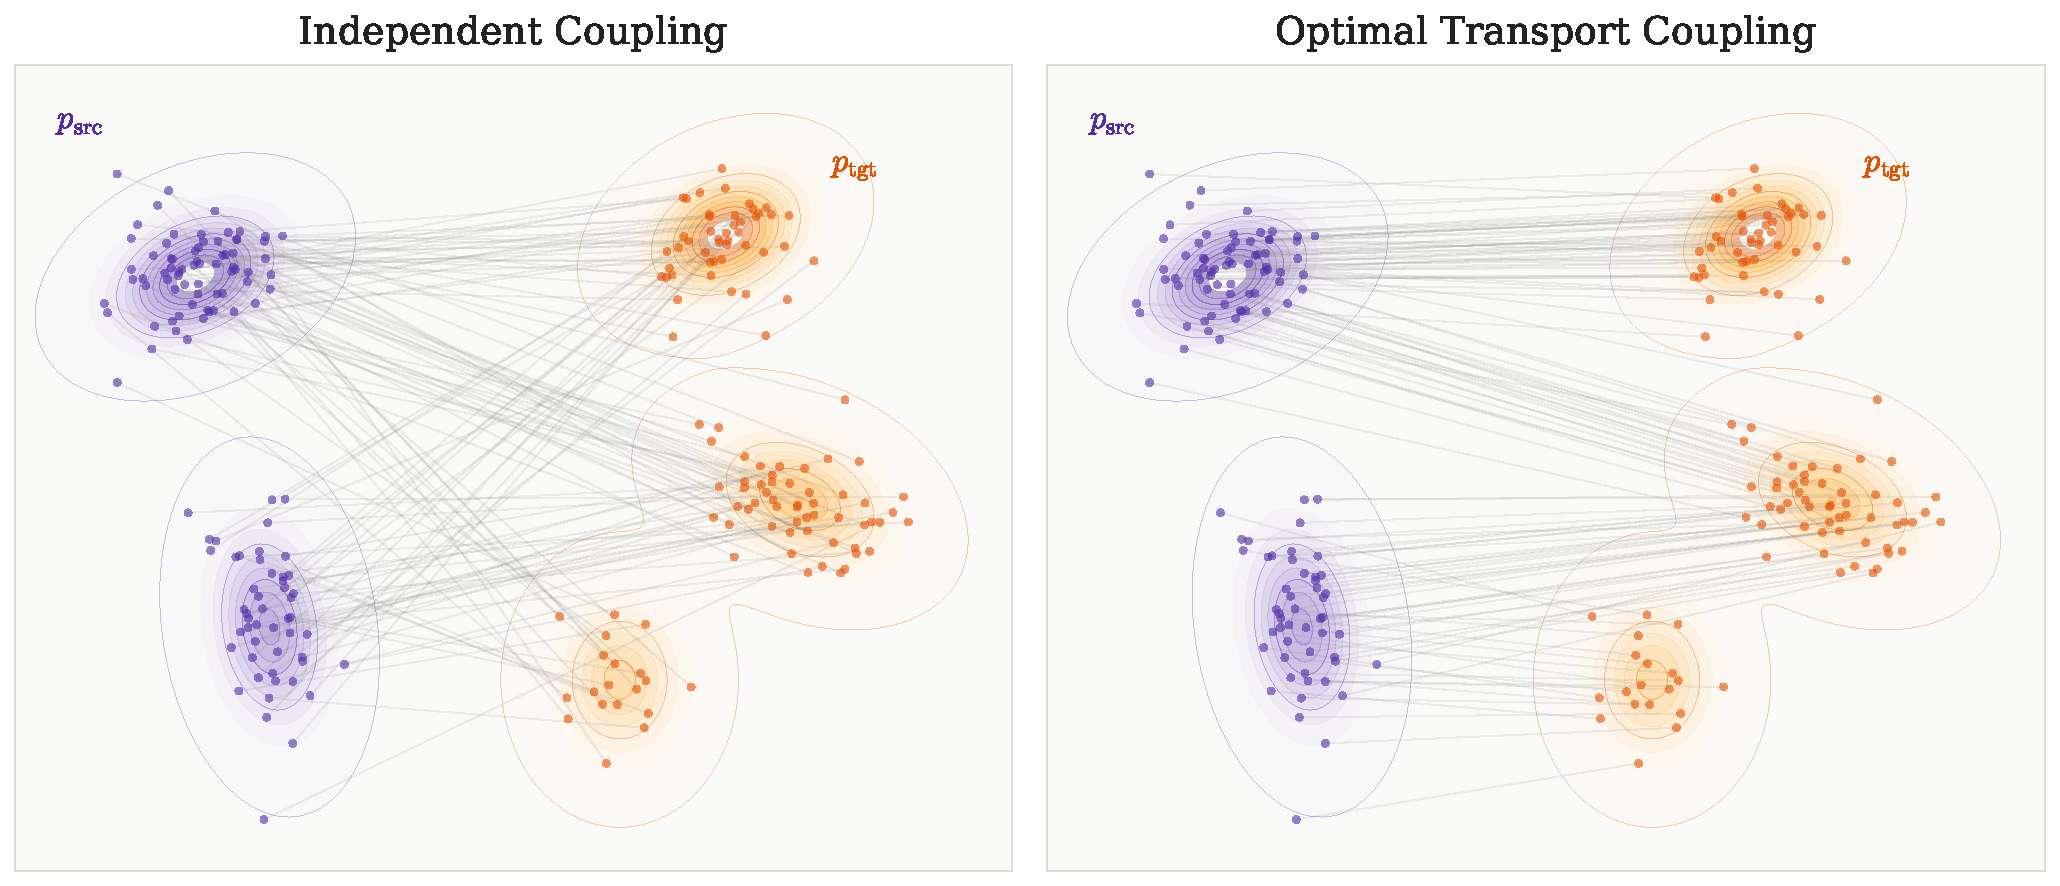
\includegraphics[width=\linewidth]{Images/PartB/ot_2d_coupling_comparison.pdf}
    \caption{\textbfs{二维中相同 $p_{\mathrm{src}}$ 和 $p_{\mathrm{tgt}}$ 之间的两种耦合。}
    左：独立（随机）配对产生交叉路径，代价较高。
    右：最优传输耦合将近处的质量配对，避免交叉。
    \figcredit{由作者在 AI 辅助编程下绘制。}}
    \label{fig:ot-2d-coupling}
\end{figure}

\paragraph{OT 问题的 Monge--Kantorovich（静态）形式。}
我们固定一个代价函数 $c:\R^D\times\R^D\to\R$，用以规定将概率质量从 $\rvx$ 发送到 $\rvy$ 的花费。目标是尽可能廉价地将源分布 $p_{\mathrm{src}}$ 变换为目标分布 $p_{\mathrm{tgt}}$。

为了定义代价，我们必须知道哪些对 $(\rvx,\rvy)$ 被匹配。这一角色由\emph{耦合}承担：它是 $\R^D\times\R^D$ 上的一个联合分布 $\gamma$，其边际分布为 $p_{\mathrm{src}}$ 和 $p_{\mathrm{tgt}}$。换言之，从 $(\rvx,\rvy)\sim\gamma$ 采样意味着我们将源中的 $\rvx$ 与目标中的 $\rvy$ 相匹配。如果 $\gamma$ 相对于勒贝格测度存在密度 $\gamma(\rvx,\rvy)$，则边际约束为
\[
\int_{\R^D} \gamma(\rvx,\rvy)\,\diff \rvy = p_{\mathrm{src}}(\rvx), 
\qquad 
\int_{\R^D} \gamma(\rvx,\rvy)\,\diff \rvx = p_{\mathrm{tgt}}(\rvy).
\]
也就是说，对 $\rvy$ 积分得到 $\rvx$ 中的源密度，而对 $\rvx$ 积分得到 $\rvy$ 中的目标密度。

我们给出两个标准示例加以说明：
\begin{enumerate}
    \item \textbfs{离散支撑。}  
    如果 $p_{\mathrm{src}}$ 和 $p_{\mathrm{tgt}}$ 支撑在有限多个点上，则一个耦合可由一个非负矩阵 $(\gamma_{ij})$ 表示，其行和等于 $p_{\mathrm{src}}(i)$，列和等于 $p_{\mathrm{tgt}}(j)$。每个元素 $\gamma_{ij}$ 是从 $i$ 发送到 $j$ 的质量数量。
    \item \textbfs{确定性映射。}  
    如果存在一个可测映射 $\rmT$ 满足 $\rmT_\#p_{\mathrm{src}}=p_{\mathrm{tgt}}$，那么
    $\gamma=(\rmI,\rmT)_\#p_{\mathrm{src}}$ 是一个确定性耦合，它将每个点
    $\rvx$ 直接移动到 $\rmT(\rvx)$。
\end{enumerate}

一旦固定了耦合 $\gamma$，传输代价就是该方案下单位代价的平均：
\[
\int c(\rvx,\rvy)\,\diff\gamma(\rvx,\rvy)
=\E_{(\rvx,\rvy)\sim\gamma}\!\big[c(\rvx,\rvy)\big].
\]
在离散情形下，它简化为 $\sum_{i,j} c_{ij}\gamma_{ij}$；在连续情形下，它变为一个二重积分。在下文中，我们将只关注连续情形。

最优传输问题即是在所有可容许耦合中，选择使该期望代价最小化的那一个。
\begin{mdframed}
\begin{equation}\label{eq:ot}
\mathrm{OT}\big(p_{\mathrm{src}},p_{\mathrm{tgt}}\big)
:= \inf_{\gamma\in\Gamma(p_{\mathrm{src}},p_{\mathrm{tgt}})}
\int c(\rvx,\rvy)\,\diff\gamma(\rvx,\rvy),
\end{equation}
\end{mdframed}
其中可行集只是施加了边际（即质量守恒）约束：
\begin{align*}
    \Gamma(p_{\mathrm{src}},p_{\mathrm{tgt}})
= \Big\{\gamma \in &\mathcal{P}(\R^D\times\R^D): \\
&\int \gamma(\rvx,\rvy) \diff \rvy = p_{\mathrm{src}}(\rvx),\,\,
\int \gamma(\rvx,\rvy)\diff \rvx = p_{\mathrm{tgt}}(\rvy)\Big\},
\end{align*}
其中 $\mathcal{P}(\R^D\times\R^D)$ 表示 $\R^D\times\R^D$ 上所有概率测度的集合。  


\subparagraph{特例：Wasserstein-2 距离。}

Wasserstein-2 距离是 Monge--Kantorovich 问题在二次代价 $c(\mathbf{x}, \mathbf{y}) = \|\mathbf{x} - \mathbf{y}\|^2$ 下的特例。它度量两个概率分布之间的距离如下：
\begin{align*}
 \mathcal{W}_2^2(p_{\mathrm{src}}, p_{\mathrm{tgt}}) := \inf_{\gamma \in \Gamma(p_{\mathrm{src}}, p_{\mathrm{tgt}})} \mathbb{E}_{(\mathbf{x}, \mathbf{y}) \sim \gamma} \left[ \|\mathbf{x} - \mathbf{y}\|^2 \right].
\end{align*}

在对 $p_{\mathrm{src}}$ 和 $p_{\mathrm{tgt}}$ 的适当假设下，Brenier 定理（见 \Cref{thm:brenier}）\footnote{Brenier 定理关于二次代价下最优传输映射的存在性与结构。特别地，如果 $p_{\mathrm{src}}$ 不赋予维数至多为 $D-1$ 的集合以质量，则最优传输映射 $\rmT^*$ 唯一存在。}保证二次代价下的最优耦合 $\gamma$ 集中于一个确定性映射 $\rmT:\mathbb{R}^D \rightarrow \mathbb{R}^D$ 的图上。因此，Wasserstein-2 距离可以等价地表示为\footnote{$\mathcal{W}_2$ 距离有三种常用形式：Monge 形式（基于最优传输映射）、Kantorovich 形式（基于耦合）以及 Benamou--Brenier 动态形式（见 \Cref{eq:bb-ot}）。在适当的正则性条件下这些形式是等价的。}：
\begin{equation}\label{eq: Monge's Formulation}    \mathcal{W}_2^2(p_{\mathrm{src}}, p_{\mathrm{tgt}}) = \inf_{\substack{\rmT:\mathbb{R}^D \rightarrow \mathbb{R}^D,\\ \text{ s.t. }\rmT\#p_{\mathrm{src}} = p_{\mathrm{tgt}}}} \mathbb{E}_{\rvx \sim p_{\mathrm{src}}} \left[ \| \rmT(\rvx) - \rvx \|^2 \right].
\end{equation}
这里 $\rmT\#p_{\mathrm{src}} = p_{\mathrm{tgt}}$ 表示 $ \rmT $ 将 $ p_{\mathrm{src}} $ 前推为 $ p_{\mathrm{tgt}} $，即当 $ \rvx \sim p_{\mathrm{src}}$ 时有 $ \rmT(\rvx) \sim p_{\mathrm{tgt}}$。 

 

因此，Wasserstein-2 距离表示在所有匹配给定边际的耦合或传输映射中，最小的期望平方传输代价。记为 $\rmT^*(\mathbf{x})$ 的最优传输映射，称为 \emph{Monge 映射}，给出了将 $p_{\mathrm{src}}$ 变换为 $p_{\mathrm{tgt}}$ 的最有效方式。

\paragraph{OT 的 Benamou--Brenier（动态）形式。} 
\begin{figure}[th!]
    \centering
    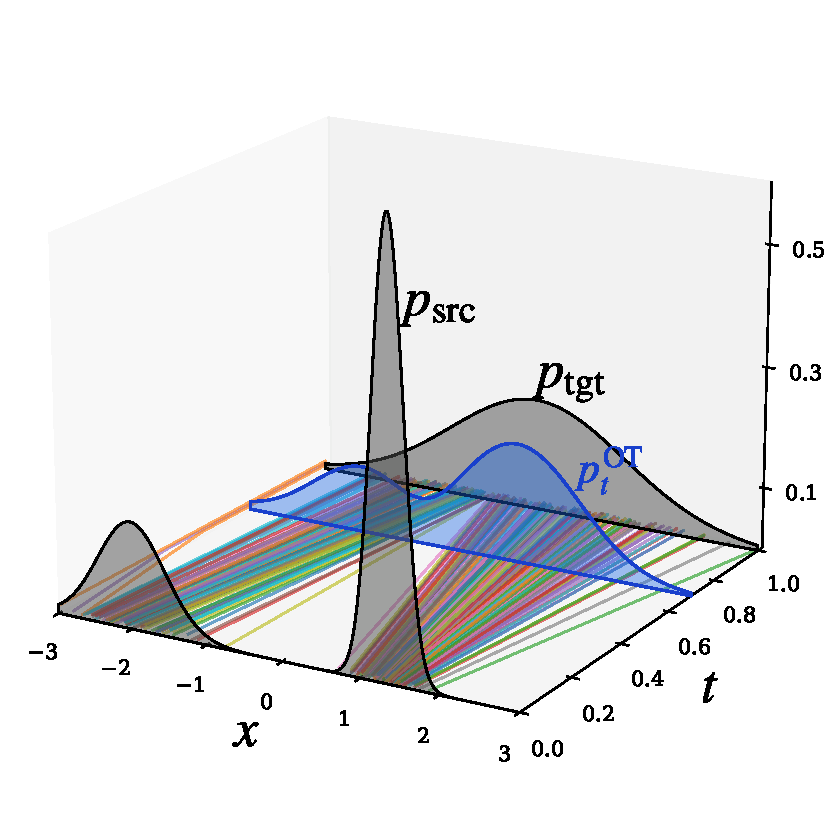
\includegraphics[width=0.8\linewidth]{Images/PartB/ot_illustration.pdf}
    \caption{ \textbfs{OT 动态视角的示意图。} 插值 $p_t^{\mathrm{OT}}$ 随时间连续演化，
提供了将 $p_{\mathrm{src}}$ 确定性地映射到 $p_{\mathrm{tgt}}$ 的最小代价传输方案（即 McCann 的位移插值）。
\figcredit{由作者绘制。}}
    \label{fig:ill-ot}
\end{figure}



不同于 Monge--Kantorovich 形式中以静态方式直接映射分布，传输也可以建模为连续时间的流：
\begin{equation*}
    p_0 := p_{\mathrm{src}} \to p_t \to p_1 := p_{\mathrm{tgt}}, \quad t \in [0,1].
\end{equation*}
这一最优传输的动态形式由 \citet{benamou2000computational} 提出，它寻求一个光滑的速度场 $ \rvv_t(\rvx) $ 来描述 $ p_t(\rvx) $ 中的质量如何随时间演化。

Benamou--Brenier 形式\footnote{Benamou–Brenier 形式描述了如何在测度与速度的连续路径上最小化动能，从而计算 $ \mathcal{W}_2 $ 距离。}表明，对于二次代价 $ c(\rvx, \rvy) = \|\rvx - \rvy\|_2^2 $（即 $ \mathcal{W}_2 $ 距离），\Cref{eq:ot} 中静态 OT 问题的最优值等于如下动能最小化问题的最优值：
%the static OT problem in \Cref{eq:ot} is equivalent \doh{``Equivalent'' is unclear.} to the following dynamic formulation:
\begin{mdframed}
   \begin{equation}\label{eq:bb-ot}
    \mathcal{W}_2^2(p_{\mathrm{src}}, p_{\mathrm{tgt}}) = \min_{\substack{ (p_t, \rvv_t) \text{ s.t. }
        \partial_t p_t + \nabla \cdot (p_t \rvv_t) = 0, \\
        p_0 = p_{\mathrm{src}},\,\, p_1 = p_{\mathrm{tgt}}
    }}
    \int_0^1 \int_{\mathbb{R}^D} \|\rvv_t(\rvx)\|^2 p_t(\rvx) \diff\rvx \diff t
\end{equation} 
\end{mdframed}
其中对每个 $t \in [0,1]$，$p_t$ 是 $\mathbb{R}^D$ 上的一个概率分布。特别地，最优传输流 $p_t(\rvx)$ 遵循 \textit{McCann 位移插值}：
\begin{equation*}
    \rmT_t^*(\rvx) = (1 - t)\rvx + t\rmT^*(\rvx),
\end{equation*}
其中 $\rmT^*(\rvx)$ 是将 $p_{\mathrm{src}}$ 传输到 $p_{\mathrm{tgt}}$ 的 OT 映射。这种线性插值使质量以常速度沿直线移动：对每个 $t \in [0,1]$ 有 $p_t = \rmT_t^*\#p_{\mathrm{src}}$。

最优传输映射 $\rmT^*$ 满足 \emph{Monge–Ampère 方程}：
%However, computing $\rmT^*$ generally requires solving the \emph{Monge–Ampère equation}:
\begin{equation}\label{eq:monge-ampere}
    p_{\mathrm{tgt}}\left(\nabla \psi(\rvx)\right) \det\left(\nabla^2 \psi(\rvx)\right) = p_{\mathrm{src}}(\rvx),
\end{equation}
其中由 Brenier 定理知，对某个凸函数 $\bpsi$ 有 $\rmT^*(\rvx) = \nabla \psi(\rvx)$。然而，这个非线性偏微分方程通常难以获得显式解。注意，这正是归一化流所使用的变量替换关系（参见 \Cref{eq:nf-change-of-var}）：流用一个具有可处理雅可比行列式的可逆传输映射进行参数化，但一般并不施加“梯度势”结构 $\rmT^*=\nabla\psi$；因此，训练得到的流可能与 Brenier/OT 映射存在显著差异。




\subsection{熵正则化最优传输（EOT）}

为了具体地引出 EOT，考虑由样本构造的经验分布。假设 $p_{\mathrm{src}}$ 支撑在点 $\{\rvx^{(i)}\}_{i=1}^n \subset \R^D$ 上且权重为 $a_i$，而 $p_{\mathrm{tgt}}$ 支撑在 $\{\rvy^{(j)}\}_{j=1}^n \subset \R^D$ 上且权重为 $b_j$。那么耦合就是一个 $n\times n$ 的非负矩阵 $\gamma=(\gamma_{ij})$，其行和匹配 $a$，列和匹配 $b$。每个元素 $\gamma_{ij}$ 表示从 $\rvx^{(i)}$ 传输到 $\rvy^{(j)}$ 的质量数量\footnote{经验（离散）测度为连续分布提供了一个有原则的代理。当地面代价为 $c(x,y)=d(x,y)^p$（从而 OT 值等于 $W_p^p$）且测度具有有限的 $p$ 阶矩时，经验测度以可量化的速率在 $W_p$ 中收敛到总体分布；参见 \citet{fournier2015rate} 以及 \citet{peyre2019computational} 中的综述。}。

\paragraph{为何要对 OT 进行正则化？}
此离散情形下的经典 OT（通过在连续形式 \Cref{eq:ot} 中取计数测度得到）归结为最小化
\[
\min_{\gamma=(\gamma_{ij})}\sum_{i,j} C_{ij}\,\gamma_{ij},
\]
约束为所有可行耦合 $\gamma=(\gamma_{ij})$，其中对于预定的地面代价 $c:\R^D\times\R^D\to\R_{\ge 0}$（例如 $c(\rvx,\rvy)=\|\rvx-\rvy\|_2^2$），$C_{ij} = c(\rvx^{(i)},\rvy^{(j)})$ 表示将一个单位质量从源点 $\rvx^{(i)}$ 移动到目标点 $\rvy^{(j)}$ 的代价。

这会产生两个主要问题：
\begin{enumerate}
    \item \textbfs{非唯一性与不稳定性：} 最小化子 $\gamma^*$ 未必唯一。例如，如果两个传输方案达到相同的最小代价，求解器可能选择其中任意一个。因此，输入 $(a,b,C)$ 的微小变化（如移动一个样本、调整权重或轻微扰动代价）都可能引起解的突变。  
    \item \textbfs{计算代价高：} 该问题是一个具有 $n^2$ 个变量和 $2n$ 个约束的线性规划。实际求解器（如匈牙利算法~\citep{kuhn1955hungarian,munkres1957algorithms}、网络单纯形法~\citep{peyre2019computational}）通常复杂度为 $\mathcal{O}(n^3)$，对大 $n$ 不可行。
\end{enumerate}

为克服这些瓶颈，EOT 目标函数在经典 OT 问题中引入了一项正则化项，由参数 $\varepsilon > 0$ 控制：
\begin{mdframed}
    \begin{align}\label{eq:eot-epsilon}
\begin{aligned}
        \text{EOT}_\varepsilon(p_{\mathrm{src}}, p_{\mathrm{tgt}}) &:= \min_{\gamma \in \Gamma(p_{\mathrm{src}}, p_{\mathrm{tgt}})} \int c(\rvx,  \rvy)  \diff\gamma(\rvx, \rvy) 
        + \varepsilon \mathcal{D}_{\text{KL}}\left(\gamma \Vert M \right).
\end{aligned}
\end{align}
\end{mdframed}
参考测度 $M$ 通常选为边际的乘积，即 $p_{\mathrm{src}} \otimes p_{\mathrm{tgt}}$。KL 散度项与传输方案 $\gamma$ 的香农熵直接相关：
\[
\mathcal{D}_{\text{KL}}(\gamma \,\Vert\, p_{\mathrm{src}} \otimes p_{\mathrm{tgt}}) = -\mathcal{H}(\gamma) + \text{Constant},
\]
其中 $\mathcal{H}(\gamma) := -\int \gamma(\rvx, \rvy) \log \gamma(\rvx, \rvy) \diff \rvx \diff \rvy$。



加入这一正则化项带来若干理论与实践上的优势，我们简要概述如下：
\paragraph{熵正则化项为何有用？}
\begin{enumerate}
  \item \textbfs{质量分散。}
  由于 $t\mapsto t\log t$ 是凸函数且对大 $t$ 增长迅速，最小化 $\int \gamma\log\gamma$
  会惩罚\emph{尖锐}耦合（某些 $\gamma(\rvx,\rvy)$ 非常大，其余接近零）。
  在总质量 $\int \gamma=1$ 固定时，它倾向于使 $\gamma(\rvx,\rvy)$ 在 $(\rvx,\rvy)\in\mathbb{R}^D\times\mathbb{R}^D$ 上分布得更均匀。
  等价地，最大化香农熵会促进更高的“不确定性”（弥散性）。

  \item \textbfs{严格凸性与唯一性。}
  由于 $\mathcal{H}$ 严格凹，\Cref{eq:eot-epsilon} 中的目标关于 $\gamma$ 严格凸，
  从而给出\emph{唯一}最小化子 $\gamma^*_\varepsilon$，且它连续依赖于 $(p_{\mathrm{src}},p_{\mathrm{tgt}},c)$。

  \item \textbfs{Sinkhorn 形式与正性。}
  在温和条件下\footnote{我们假设 $c<\infty$ 在 $p_{\mathrm{src}}\otimes p_{\mathrm{tgt}}$-几乎处处成立，并且边际核积分有限且为正。为简单起见，我们聚焦于 $\gamma^*_\varepsilon$、$p_{\mathrm{src}}$ 与 $p_{\mathrm{tgt}}$ 相对于勒贝格测度均存在密度的情形。
},
  最优解具有 \emph{Schrödinger/Sinkhorn 形式}
  \[
  \gamma^*_\varepsilon(\rvx,\rvy) = u(\rvx)\, \exp \bigl(-\tfrac{c(\rvx,\rvy)}{\varepsilon}\bigr)  \,v(\rvy)p_{\mathrm{src}}(\rvx) p_{\mathrm{tgt}}(\rvy),
  \]
  其中 $u,v$ 为正的缩放函数（在相差一个全局常数因子下唯一）。实践中，连续形式用有限样本近似，从而将 EOT 归约为有限（采样的）Sinkhorn 迭代。
该熵正则化目标严格凸，缩放（Sinkhorn/IPFP）算法可高效求解~\citep{sinkhorn1964relationship,cuturi2013sinkhorn}。
对于每个边际有 $n$ 个支撑点（即 $n\times n$ 核）的稠密问题，每次 Sinkhorn 迭代的时间与内存均为 $\mathcal{O}(n^2)$，
使该方法更具可扩展性和实用性~\citep{altschuler2017near}。

  \item \textbfs{$\varepsilon$ 的极限。}
当 $\varepsilon \to 0$ 时，最优方案 $\gamma^*_\varepsilon$ 越来越集中，逼近（可能奇异的）经典 OT 耦合（我们将在 \Cref{subsec:eot-ot} 中重新审视这一联系）。
当 $\varepsilon$ 增大时，$\gamma^*_\varepsilon$ 逐渐铺展开来，并逼近独立耦合 $p_{\mathrm{src}}\otimes p_{\mathrm{tgt}}$。
\end{enumerate}



\subsection{薛定谔桥（SB）}\label{subsec:sb}


\paragraph{SB 的 KL 形式。}
薛定谔桥（SB）问题由 Erwin Schrödinger 于 20 世纪 30 年代提出，它提出如下问题。假设粒子按某种简单的参考动力学（例如布朗运动）运动。现在设想我们在两个时刻观测粒子：在 $t=0$ 时其分布为 $p_{\mathrm{src}}$，在 $t=1$ 时为 $p_{\mathrm{tgt}}$。在所有连接这两个分布的随机过程中，哪一个偏离参考动力学最小？这里“偏离”由 KL 散度度量，因此 SB 问题的解是将布朗运动变形为满足预定边界条件的过程的最可能方式。

为使其精确化，令 $\rvx_{0:T}:=\{\rvx_t\}_{t\in[0,T]}$ 表示过程的一条完整轨迹。我们用 $P$ 表示\emph{轨迹的律}（law），即整个样本路径上的概率分布。$P$ 的时间 $t$ 边际记为 $p_t$（或 $P_t$），它描述单个时刻状态 $\rvx_t$ 的分布。形式上，对于可测集 $A\subseteq\mathbb R^D$，
\[
p_t(A) = P(\rvx_t \in A).
\]
换言之，$p_t$ 可视为如下的经验分布：从 $P$ 中采样许多条完整轨迹，然后收集 $t$ 时刻的状态——例如，当状态为一维时表现为直方图。


考虑一个由如下 SDE 驱动的参考扩散 $\{\rvx_t\}_{t\in[0,T]}$
\begin{align}\label{eq:general-sb-sde}
    \diff \rvx_t  =  \rvf(\rvx_t,t)\,\diff t  +  g(t)\,\diff \rvw_t,
\end{align}
其中 $\rvf\colon \R^D\times[0,T]\!\to\!\R^D$，$g\colon[0,T]\!\to\!\R$，且
$\{\rvw_t\}_{t\in[0,T]}$ 是标准布朗运动。  
记 $R$ 为完整轨迹
$\rvx_{0:T}:=\{\rvx_t\}_{t\in[0,T]}$ 的\emph{路径律}（联合分布）；这个 $R$ 将作为\emph{参考}轨迹分布。

采用上述记号，SB 问题寻求一个轨迹律 $P$，使其在 KL 散度下最接近 $R$，同时匹配预定的端点边际：
\begin{align}\label{eq:sb-epsilon-general}
    \mathrm{SB}(p_{\mathrm{src}}, p_{\mathrm{tgt}})
    := \min_{P}\, \mathcal{D}_{\mathrm{KL}}(P\|R)
    \quad \text{s.t.} \quad P_0 = p_{\mathrm{src}},\;\; P_T = p_{\mathrm{tgt}}.
\end{align}
最优解 $P^*$ 依赖于所选的参考过程 $R$。

\paragraph{SB 的随机控制视角。}

\begin{figure}[th!]
    \centering
    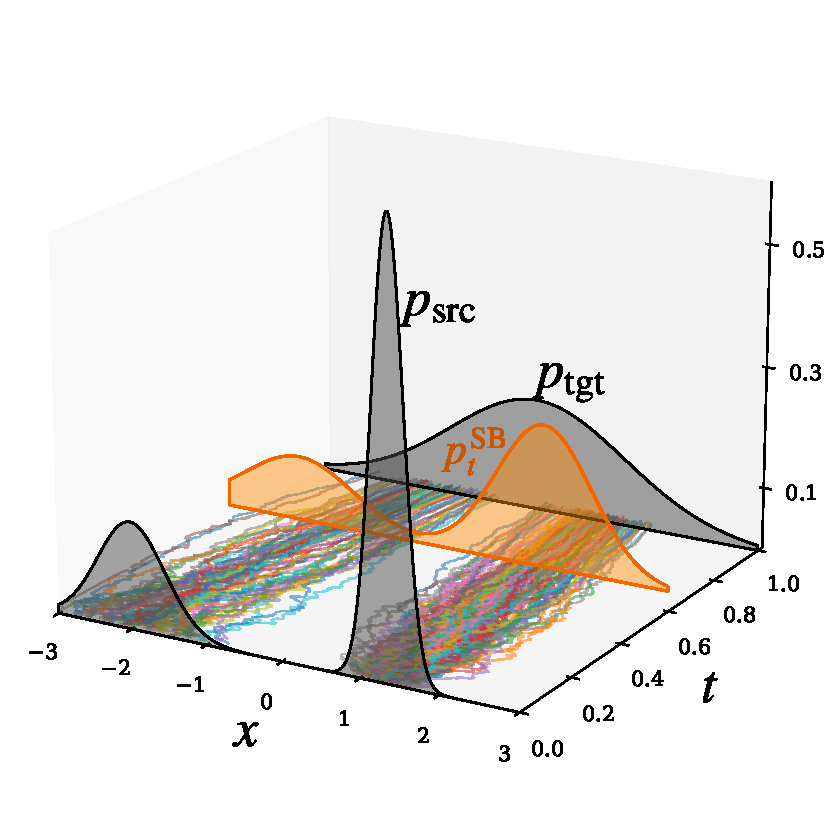
\includegraphics[width=0.8\linewidth]{Images/PartB/sb_illustration.pdf}
    \caption{\textbfs{SB 的随机控制视角示意图。} 该桥寻求在连接 $p_{\mathrm{src}}$ 与 $p_{\mathrm{tgt}}$ 的同时偏离参考最少的随机路径。
    \figcredit{由作者绘制。}}
    \label{fig:ill-sb}
\end{figure}


与其在 \Cref{eq:sb-epsilon-general} 中对任意路径分布 $P$ 进行优化，一种更易处理的途径是将参考动力学作为锚点并允许其漂移。这通过引入一个随时间变化的漂移 $\rvv_t(\rvx_t)$ 来实现，它扰动参考过程并生成一族候选轨迹分布。所得动力学具有\emph{受控扩散}的形式：
\[
    \diff \rvx_t
    = \bigl[\rvf(\rvx_t,t) + \rvv_t(\rvx_t)\bigr]\diff t + g(t) \diff \rvw_t,
\]
其中 $\rvv_t:\R^D\to\R^D$ 是待后优化的漂移（\Cref{eq:sb-kinetic}）。 在标准的可积性条件（如 Novikov 条件）下，并由 Girsanov 定理
（见 \Cref{subsec:girsanov}），受控律 $P$ 与参考 $R$ 之间的 KL 散度具有动态（动能）形式
\begin{align*}
    \mathcal{D}_{\mathrm{KL}}(P\|R)
    = \E_{P}\!\left[\frac{1}{2}\int_0^T \frac{\|\rvv_t(\rvx_t)\|^2}{g^2(t)} \diff t\right]
    = \frac{1}{2}\int_0^T\!\int_{\R^D}\frac{\|\rvv_t(\rvx)\|^2}{g^2(t)} p_t(\rvx) \diff \rvx \diff t,
\end{align*}
其中 $p_t$ 是受控过程下 $\rvx_t$ 的时间 $t$ 边际。第二个等式由全期望公式得到。

因此，SB 问题可重新表述为：在所有将过程从 $t=0$ 处的 $p_{\mathrm{src}}$ 驾驭到 $t=T$ 处 $p_{\mathrm{tgt}}$ 的可容许漂移 $\rvv_t$ 上，最小化期望控制能量
\citep{dai1991stochastic,pra1990markov,pavon1991free,chen2016relation}。这导出\emph{随机控制形式}：
\begin{mdframed} 
\begin{align}\label{eq:sb-kinetic} 
\begin{aligned} &\mathrm{SB}_\varepsilon(p_{\mathrm{src}}, p_{\mathrm{tgt}}) \\= & \min_{\substack{ \mathbf{v}_t \text{ s.t. } \diff \rvx_t = \left[\rvf(\rvx_t, t) + \mathbf{v}_t(\rvx_t) \right]\diff t + g(t) \diff \rvw_t, \\ \rvx_0 \sim p_{\mathrm{src}}, \,\, \rvx_T \sim p_{\mathrm{tgt}} }} \frac{1}{2} \int_0^T\int_{\mathbb{R}^D} \frac{\norm{\rvv_t(\rvx)}^2}{g^2(t)} p_t(\rvx)\diff \rvx \diff t, 
\end{aligned}
\end{align} 
\end{mdframed}

重要的是，端点分布 $p_{\mathrm{src}}$ 和 $p_{\mathrm{tgt}}$ 是任意的；
控制 $\rvv_t$ 的选择正是为了在这些边际之间“桥接”参考动力学，同时尽可能（在 KL 散度下）接近参考过程 $R$。

\paragraph{特殊的布朗参考。}
\Cref{eq:sb-kinetic} 类似于 \Cref{eq:bb-ot} 中 OT 的 Benamou--Brenier 形式，尤其当参考过程 $R^\varepsilon$（$\varepsilon>0$）选为布朗
运动\footnote{这种相似性可以严格化。在一种等价的时间对称流体动力学形式中，若 $\tilde{\rvv}_t$ 表示满足连续性方程
$\partial_t \rho_t + \nabla \cdot (\rho_t \tilde{\rvv}_t)=0$ 的当前速度，则布朗参考 SB 目标（\Cref{eq:sb-epsilon-kinetic}）可
写为 Benamou--Brenier 型动能项（至多差一个约定常数因子）加上一个 Fisher 信息项：
\[
\int_0^T\!\!\int
\left[
\frac{1}{2}\|\tilde{\rvv}_t(\rvx)\|^2
+
\frac{\varepsilon^2}{8}\|\nabla_{\rvx}\log \rho_t(\rvx)\|^2
\right]\rho_t(\rvx)\,\diff\rvx\,\diff t.
\]
因此，在布朗参考 / 二次代价情形下，熵正则化最优传输可视为动态 OT 的 Fisher 信息正则化版本；参见
\citet{chen2021stochastic} 中的问题 4.6。}：
\[
\diff \rvx_t = \sqrt{\varepsilon}\,\diff\rvw_t,
\]
从而 $\rvf \equiv \mathbf{0}$ 且 $g(t) \equiv \sqrt{\varepsilon}$。

在此设定下，SB 问题寻求一个在 KL 散度下最接近布朗参考 $R^\varepsilon$ 的路径分布 $P$，同时匹配端点边际：
\begin{align}\label{eq:sb-epsilon}
    \mathrm{SB}_\varepsilon(p_{\mathrm{src}}, p_{\mathrm{tgt}})
    := \min_{P} \mathcal{D}_{\mathrm{KL}}(P \| R^\varepsilon)
    \quad \text{s.t.} \quad P_0 = p_{\mathrm{src}}, \;\; P_T = p_{\mathrm{tgt}}.
\end{align}
等价的随机控制形式则变为
\begin{align}\label{eq:sb-epsilon-kinetic}
\begin{aligned}
    \mathrm{SB}_\varepsilon(p_{\mathrm{src}}, p_{\mathrm{tgt}})
    = \min_{\substack{
        \rvv_t \text{ s.t. } \diff \rvx_t = \rvv_t(\rvx_t)\,\diff t + \sqrt{\varepsilon}\,\diff \rvw_t, \\
        \rvx_0 \sim p_{\mathrm{src}},\;\; \rvx_T \sim p_{\mathrm{tgt}}
    }}
    \frac{1}{2\varepsilon}\int_0^T \!\!\int_{\R^D}
        \|\rvv_t(\rvx)\|^2 \, p_t(\rvx)\,\diff \rvx\,\diff t,
\end{aligned}
\end{align}
其中 $p_t$ 表示由漂移 $\rvv_t$ 驱动的扩散的时间 $t$ 边际：
\[
\diff \rvx_t = \rvv_t(\rvx_t)\,\diff t + \sqrt{\varepsilon}\,\diff \rvw_t.
\]



\paragraph{为何需要指定参考分布？} 
与经典 OT 不同，SB 问题由于其随机性而需要一个参考分布。在 OT 中，代价函数（例如 $c(\rvx, \rvy) \propto \|\rvx - \rvy\|^2$）隐式地定义了唯一的确定性测地线路径，使参考变得不必要。相反，SB 设定允许无穷多个连接边际的随机过程，且没有内在的“自然”路径概念。参考测度 $R$ 编码了系统潜在的物理或几何结构（例如布朗运动），并定义了基于 KL 的优化目标 $\mathcal{D}_{\mathrm{KL}}(P \| R)$，否则最优性的概念便无法定义。



\paragraph{耦合 PDE 刻画。}  
描述 SB 解的一种便捷方式是借助两个时空势 $\Psi(x,t)$ 和 $\widehat{\Psi}(x,t)$。令
$p_t^{\mathrm{SB}}$ 表示 \Cref{eq:sb-epsilon-general} 中最优轨迹律 $P^*$ 在时间 $t\in[0,T]$ 处的边际。则有如下对称分解~\citep{dai1991stochastic}
\begin{align}\label{eq:sb-symmetry}
p_t^{\mathrm{SB}}(x) = \Psi(x,t) \widehat{\Psi}(x,t),
\end{align}
其中 $\Psi$ 和 $\widehat{\Psi}$ 求解（线性的）\emph{Schrödinger 方程组}~\citep{caluya2021wasserstein,chen2021stochastic,chenlikelihood}：
\begin{align}
\begin{aligned}\label{eq:pde-schrodinger}
\frac{\partial \Psi}{\partial t}(\mathbf{x},t)
  &= -\nabla_{\mathbf{x}} \Psi(\mathbf{x},t) \cdot \rvf(\mathbf{x},t)
     - \frac{g^2(t)}{2}\,\Delta_\mathbf{x} \Psi(\mathbf{x},t),  \\
\frac{\partial \widehat{\Psi}}{\partial t}(\mathbf{x},t)
  &= -\nabla_{\mathbf{x}}\!\cdot\!\bigl(\widehat{\Psi}(\mathbf{x},t)\,\rvf(\mathbf{x},t)\bigr)
     + \frac{g^2(t)}{2}\,\Delta_\mathbf{x}\widehat{\Psi}(\mathbf{x},t) 
\\[4pt] \text{subject to}  \\[4pt]
\Psi(\mathbf{x},0)&\,\widehat{\Psi}(\mathbf{x},0) = p_{\mathrm{src}}(\mathbf{x}),
\quad
\Psi(\mathbf{x},T)\,\widehat{\Psi}(\mathbf{x},T) = p_{\mathrm{tgt}}(\mathbf{x}). 
\end{aligned}
\end{align}

\iffalse

\begin{align}
\begin{aligned}\label{eq:pde-schrodinger}
\frac{\partial \Psi}{\partial t}(\mathbf{x},t)
  &= -\nabla_{\mathbf{x}} \Psi(\mathbf{x},t)^\top\,\rvf(\mathbf{x},t)
     - \frac{1}{2}\,\mathrm{Tr}\bigl(g^2(t)\,\nabla_{\mathbf{x}}^2\Psi(\mathbf{x},t)\bigr),  \\
\frac{\partial \widehat{\Psi}}{\partial t}(\mathbf{x},t)
  &= -\nabla_{\mathbf{x}}\!\cdot\!\bigl(\widehat{\Psi}(\mathbf{x},t) \rvf(\mathbf{x},t)\bigr)
     + \frac{1}{2} \mathrm{Tr}\bigl(g^2(t)\,\nabla_{\mathbf{x}}^2\widehat{\Psi}(\mathbf{x},t)\bigr) 
\\[4pt] \text{subject to}  \\[4pt]
\Psi(\mathbf{x},0)& \widehat{\Psi}(\mathbf{x},0) = p_{\mathrm{src}}(\mathbf{x}),
\quad
\Psi(\mathbf{x},T) \widehat{\Psi}(\mathbf{x},T) = p_{\mathrm{tgt}}(\mathbf{x}). 
\end{aligned}
\end{align}
\fi

\subparagraph{正向时间的薛定谔桥 SDE。}
一旦已知 $\Psi$，最优动力学即是被时空因子 $\Psi$ 倾斜后的参考扩散：
\begin{align}\label{eq:sb-forward-sde}
    \diff \rvx_t = \bigl[\rvf(\rvx_t, t) + g^2(t)\,\nabla_{\mathbf{x}} \log \Psi(\rvx_t, t)\bigr]\diff t
+ g(t)\diff \rvw_t, \quad \rvx_0 \sim p_{\mathrm{src}}.
\end{align}
令 $Q$ 表示 \Cref{eq:sb-forward-sde} 的轨迹律
（故由 \Cref{eq:sb-symmetry,eq:pde-schrodinger} 知 $Q_0=p_{\mathrm{src}}$ 且 $Q_T=p_{\mathrm{tgt}}$）。则
\emph{$Q=P^*$} 且 \Cref{eq:sb-kinetic} 的最小化子 $\rvv^*$ 为（见 \citep{chen2021stochastic} 的第 4.6 节）： 
\[
\rvv_t^{*}(\rvx) = g^2(t) \nabla_\rvx \log \Psi(\rvx,t).
\]
也就是说，
漂移校正 $g^2\nabla_\rvx\log\Psi$ 恰好是为匹配端点边际而对参考施加的
最小 KL 扰动。

%\textcolor{red}{In other words, the optimal control $\mathbf{v}_t(\rvx_t)$ of the stochastic control formulation \Cref{eq:sb-kinetic} of SB is given by
%\begin{align*}
%    \mathbf{v}_t(\rvx_t) = \rvf(\rvx_t, t) + g^2(t)\,\nabla_{\mathbf{x}} \log \Psi(\rvx_t, t).
%\end{align*}
%}

\subparagraph{逆向时间的薛定谔桥 SDE。}
同一个最优路径律也可以在时间上逆向生成。考察逆向时间漂移形式的一种便捷方式是，在概念上使用扩散的标准时间反演恒等式：
\[
\rvb^{-}(\rvx,t)=\rvb^{+}(\rvx,t)-g^2(t)\nabla_\rvx\log p_t^{\mathrm{SB}}(\rvx),
\]
其中 $\rvb^{+}=\rvf+g^2\nabla\log\Psi$ 且 $p_t=\Psi\,\widehat{\Psi}$。这给出
\[
\rvb^{-}(\rvx,t)=\rvf(\rvx,t)-g^2(t) \nabla_\rvx\log \widehat{\Psi}(\rvx,t).
\]
于是逆向时间 SDE 为
\begin{align}\label{eq:sb-backward-sde}
\diff \rvx_t
= \Big[\rvf(\rvx_t,t) - g^2(t) \nabla_{\rvx}\log \widehat{\Psi}(\rvx_t,t)\Big]\diff t
+ g(t)\,\diff \bar{\rvw}_t, \quad \rvx_T \sim p_{\mathrm{tgt}} .
\end{align}
等价地，通过 $\rvy_\tau := \rvx_{T-\tau}$ 重新参数化时间，使
$\tau$ 从 $0$ 增加到 $T$。则 $\rvy_\tau$ 在 $\tau$ 上正向演化，从 $\rvy_0 \sim p_{\mathrm{tgt}}$ 出发，演化为
\begin{align}\label{eq:sb-reverse-forward-tau}
\begin{aligned}
    \diff \rvy_\tau
= \big[-\rvf(\rvy_\tau,T-\tau) + g^2(T-\tau) \nabla_{\rvy}\log \widehat{\Psi}(\rvy_\tau,&T-\tau)\big]\diff \tau
\\&+ g(T-\tau) \diff \rvw_\tau.
\end{aligned}
\end{align}
在 \Cref{eq:sb-kinetic} 的逆向时间随机控制形式中（采用相同的二次能量，但时钟反转）：
\begin{align}
\min_{\substack{
\rvu_\tau \text{ s.t. }  
\diff \rvy_\tau = \left[-\rvf(\rvy_\tau,T-\tau)+\rvu_\tau(\rvy_\tau)\right]\diff\tau
+ g(T-\tau) \diff \rvw_\tau,\\
\rvy_0 \sim p_{\mathrm{tgt}},\ \rvy_T \sim p_{\mathrm{src}}
}}
\tfrac12 \int_{0}^{T} \int_{\R^D} \tfrac{\|\rvu_\tau(\rvy)\|^2}{g^2(T-\tau)}\,p_{T-\tau}(\rvy)  \diff\rvy \diff\tau .
\end{align}
最优控制为
\[
\rvu_\tau^{*}(\rvy)=g^2(T-\tau)\nabla_{\rvy}\log\widehat{\Psi}(\rvy,T-\tau).
\]



正向与逆向描述都给出相同的最优路径律 $P^*$，二者由如下关系联系
\[
\nabla\log p_t^{\mathrm{SB}}=\nabla\log\Psi+\nabla\log\widehat\Psi,
\qquad
\rvb^{-}=\rvb^{+}-g^2\,\nabla\log p_t^{\mathrm{SB}},
\]
因此它们的边际在每个时刻都与 $p_t^{\mathrm{SB}}$ 一致。  附加漂移项 $g^2\nabla\log\Psi$（正向）和
$-\,g^2\nabla\log\widehat{\Psi}$（逆向）充当控制力，在保持与参考的相对熵最接近的同时，
驾驭参考扩散以匹配端点边际。




\subparagraph{耦合 PDE 方法的实际障碍。}
为了基于 \Cref{eq:sb-backward-sde} 构造生成过程，必须求解 \Cref{eq:pde-schrodinger} 中的耦合 PDE 以获得逆向薛定谔势 $\widehat{\Psi}$。然而，这些 PDE 即使在低维设定下也以难解著称，这使得它们在生成建模中的直接应用充满挑战。为绕开这一困难，已有若干工作提出了替代策略：利用 Score SDE 技术迭代地求解每个半桥问题（$p_{\mathrm{tgt}} \leftarrow p_{\mathrm{src}}$ 和 $p_{\mathrm{tgt}} \rightarrow p_{\mathrm{src}}$）~\citep{de2021diffusion}；优化代理似然界~\citep{chenlikelihood, liu20232}；或基于样本对 $(\rvx_0, \rvx_T) \sim p_{\mathrm{src}} \otimes p_{\mathrm{tgt}}$ 的后验 $\rvx_t \vert \rvx_0, \rvx_T$ 的解析解设计免仿真训练~\citep{liu20232}。我们在此不深入技术细节，而是在 \Cref{sec:dm-and-sb} 中简要讨论扩散模型与 SB 之间的联系。

\subsection{全局前推与局部动力学：DGM 的 OT 类比}
从最优传输视角（\Cref{eq:ot}）出发，可以利用深度生成模型学习一个从简单先验到数据的传输（前推）映射，即 
$\rmG_{\bm{\phi}\#}p_{\mathrm{prior}} \approx p_{\mathrm{data}}$。 
尽管 $\rmG_{\bm{\phi}}$ 一般并不与最优传输映射重合
（除了在适当条件下施加 OT 目标的工作~\citep{genevay2018learning,onken2021ot}），
Benamou--Brenier 形式（\Cref{eq:bb-ot}）提供了一个互补的动态视角。
它不是直接学习单个全局映射，而是将传输描述为由随时间变化的局部向量场生成的连续流，在 $p_{\mathrm{prior}}$ 与 $p_{\mathrm{data}}$ 之间描绘出一条光滑路径。
这一动态形式与静态薛定谔桥问题（\Cref{eq:sb-epsilon-general}）及其随机控制对应物（\Cref{eq:sb-kinetic}）之间的关系相平行，
其中最优耦合实现为一个受控扩散过程。
生成建模中也出现了类似的类比：
诸如 GAN 或 VAE 的标准 DGM 学习一个全局前推映射，
而扩散模型学习一个驱动生成动力学的、随时间变化的局部向量场。




\newpage
\section{不同最优传输形式之间的关系}\label{sec:relation-ot}

\begin{figure}[ht!]
\centering
%In EOT and OT, the cost function is typically quadratic: $c(\rvx, \rvy)\propto\norm{\rvx-\rvy}_2^2$.}
\resizebox{\textwidth}{!}{% <-- REMOVED
\begin{tikzpicture}[
    node distance=2.2cm and 1.2cm,  % <-- REDUCED spacing
    block/.style={
        rectangle, draw, thick, rounded corners,
        fill=white!10, text width=13em,   % <-- REDUCED text width
        minimum height=5em, align=center, font=\normalsize % <-- CHANGED font to normalsize
    },
    arrow/.style = {ultra thick, -{Stealth[length=4mm, width=4mm]}},
    dashed_arrow/.style={-Latex, ultra thick, dashed, color=gray, -{Stealth[length=4mm, width=4mm]}},
    label/.style={midway, font=\small, align=center}
]

% Nodes
\node[block, text width=11em] (sde) {
    {\large \textbfs{SB}$_\varepsilon$ \\ \textbfs{（随机控制）}}\\[0.6em] 
见 \Cref{eq:sb-epsilon-kinetic}。
};

\node[block, text width=11em, below=of sde] (ode) {
   {\large \textbfs{OT} \\ \textbfs{（动态形式）}
   \\ [0.5em]
见 \Cref{eq:bb-ot}。
   }
};

\node[block, text width=11em, right=of sde, xshift=1.5cm] (sb) {
    {\large \textbfs{SB}$_\varepsilon$ \\ \textbfs{（静态形式）}}\\[0.5em]
$\displaystyle
\min_{\substack{P :\, P_0 = p_{\rm src} \\ \phantom{P :\, } P_T = p_{\rm tgt}}}
  \mathcal{D}_\mathrm{KL}(P \| R^\varepsilon)
$
};

\node[block, right=of sb, xshift=1.5cm] (eot) {
    {\large \textbfs{EOT}$_\varepsilon$ }\\[0.5em]
    $\displaystyle
        \min_{\gamma \in \Gamma(p_{\rm src}, p_{\rm tgt})}
        \int \norm{\rvx-\rvy}_2^2  \diff\gamma
         + \varepsilon  \mathcal{D}_{\mathrm{KL}}(\gamma \| p_{\rm src} \otimes p_{\rm tgt})
    $

};

\node[block, below=of eot] (ot) {
 {\large \textbfs{OT \\ （静态形式）} }\\[0.6em]
    $\displaystyle
        \min_{\gamma \in \Gamma(p_{\rm src}, p_{\rm tgt})}
        \int \norm{\rvx-\rvy}_2^2 \diff\gamma
    $
};

% Arrows using the new 'label' style
\draw[arrow] (sde) -- (ode)
    node[label, left]
    {$\varepsilon \to 0$}
    node[label, right]
    {(iv)};
\draw[arrow,<->] (sde.east) -- (sb.west)
  node[pos=.5, above, text width=9em, align=center, sloped]
    {\footnotesize$p_t = P^*(\rvx_t \in \cdot)$}
  node[pos=.5, below, text width=9em, align=center, sloped]{(i)};
\draw[arrow,<->] (sb.east) -- (eot.west)
  node[pos=.5, above, text width=8em, align=center, sloped]
    {端点投影\\ \footnotesize$\gamma^* = (\rvx_0,\rvx_T)_\# P^*$}
  node[pos=.5, below, text width=9em, align=center, sloped]
    {(ii)};
\draw[arrow] (eot) -- (ot)
    node[label, left]
    {$\varepsilon \to 0$}
    node[label, right]
    {(iii)};
\draw[arrow, <->] (ode) -- ([yshift=0.3cm] ot.west)
    node[label, below]
    {$p_t = \bPsi_t\#\gamma^*$ 其中 $\bPsi_t(\rvx,\rvy) = (1-t) \rvx + t \rvy$};
    
\end{tikzpicture}
}
\caption{\textbfs{最优传输各变体之间的关系，其中 $c(\rvx,\rvy)=\|\rvx-\rvy\|_2^2$，SB 中的参考为 $R^\varepsilon$。}
我们总结如下等价关系：(i) $\mathrm{SB}_\varepsilon$（随机控制）$\Leftrightarrow$ $\mathrm{SB}_\varepsilon$（静态形式），其中 $p_t$ 是路径测度 $P$ 的时间 $t$ 边际；(ii) $\mathrm{SB}_\varepsilon$（静态形式）$\Leftrightarrow$ $\mathrm{EOT}_\varepsilon$（见 \Cref{subsec:sb-eot}）；(iii) $\mathrm{EOT}_\varepsilon$（静态形式）$\Leftrightarrow$ $\mathrm{OT}_\varepsilon$（静态）（见 \Cref{subsec:eot-ot}）；(iv) $\mathrm{SB}_\varepsilon$（随机控制）$\Leftrightarrow$ $\mathrm{OT}$（动态）（见 \Cref{subsec:sb-ot}）。\Cref{fig:eot-epsilon} 同时可视化了联系~(iii) 和~(iv)：
随着 $\varepsilon$ 减小，耦合与传输路径都从随机 SB 区域收敛到确定性 OT。
\figcredit{由作者绘制。}} 
\label{fig:ot-dm}
\end{figure}


在深入技术细节之前，先澄清最优传输及其熵正则化的不同形式之间如何联系会很有帮助。在高层次上，这些问题可以视为相互关联的（其关联图见 \Cref{fig:ot-dm}）：
\begin{enumerate}
    \item[(i)]  以布朗运动给定的特定参考 $R^\varepsilon$ 的 SB 问题 $\mathrm{SB}_\varepsilon$
\[
\diff \rvx_t = \sqrt{\varepsilon}\,\diff \rvw_t
\]
等价于其静态形式：演化的边际 $p_t$ 恰好是最优路径测度 $P$ 的时间 $t$ 切片（见 \Cref{subsec:sb}）；
    \item[(ii)] $\mathrm{SB}_\varepsilon$ 的静态形式直接联系到熵正则化最优传输问题 $\mathrm{EOT}_\varepsilon$（见 \Cref{subsec:sb-eot}）；
    \item[(iii)] $\mathrm{EOT}_\varepsilon$ 反过来可以关联到熵正则化最优传输的静态形式 $\mathrm{OT}_\varepsilon$（见 \Cref{subsec:eot-ot}）；
    \item[(iv)] $\mathrm{SB}_\varepsilon$ 的随机控制视角也可以联系到经典 OT 的动态形式（见 \Cref{subsec:sb-ot}）。  
\end{enumerate}


这些非平凡的关系共同提供了一个跨越随机控制、熵正则化以及经典 OT 框架的紧凑视角。




\begin{figure}[th!]
    \centering
    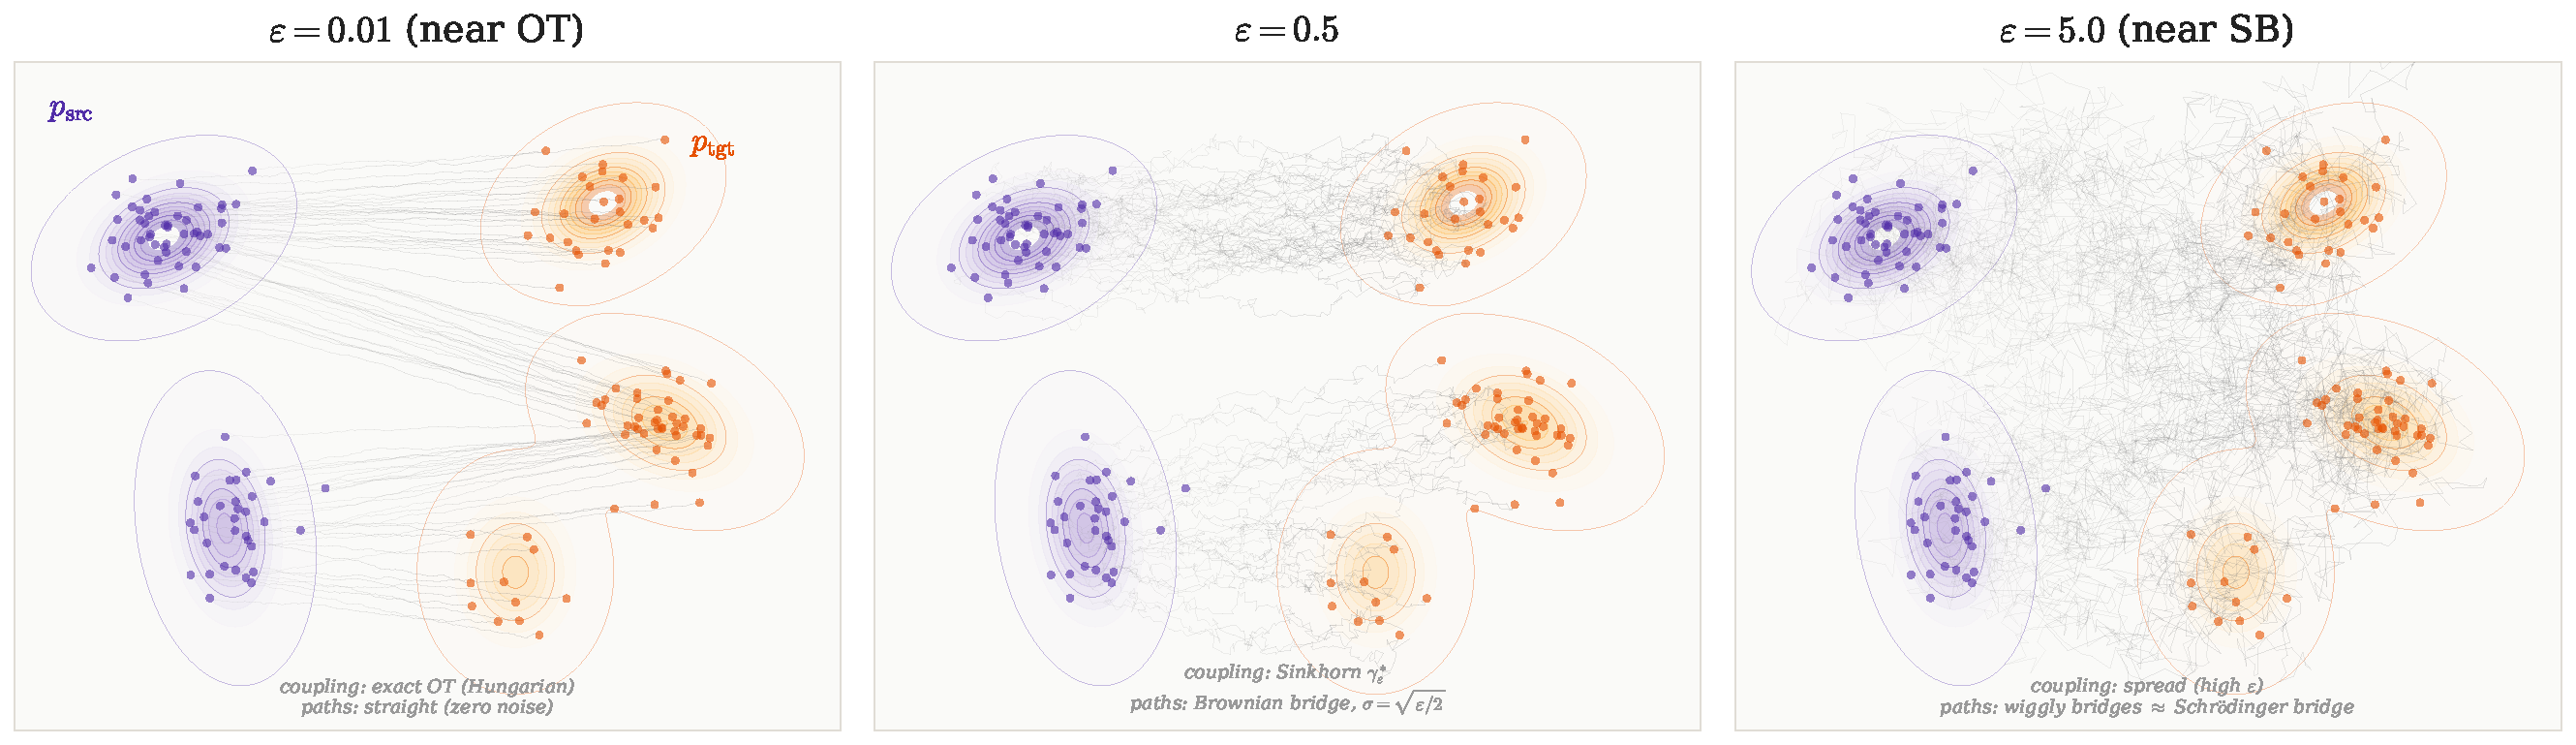
\includegraphics[width=\linewidth]{Images/PartB/eot_epsilon_interpolation.pdf}
    \caption{\textbfs{正则化参数 $\varepsilon$ 对熵正则化最优传输的影响（联系 (iii) 和 (iv)）。}
    随着 $\varepsilon$ 增大，两件事同时发生：
    耦合 $\gamma^*_\varepsilon$ 将质量铺展到更远的目标，
    传输路径也变得越来越随机。
    左（$\varepsilon=0.01$）：路径几乎为直线，每个源点映射到单一邻近目标，恢复经典 OT。
    中（$\varepsilon=0.5$）：路径出现可见波动，耦合开始铺展。
    右（$\varepsilon=2.5$）：路径高度随机，
    逼近薛定谔桥区域；
    在极限 $\varepsilon\to\infty$ 下，耦合退化为
    独立乘积 $p_{\mathrm{src}}\otimes p_{\mathrm{tgt}}$。
    耦合通过 Sinkhorn 算法计算
    （$\varepsilon\to 0$ 时用匈牙利算法）；
    在端点给定的条件下，路径是布朗桥，
    扩散系数 $\sigma=\sqrt{\varepsilon/2}$，
    来自 Mikami 对偶（\Cref{subsec:sb-eot}）。
    \figcredit{由作者在 AI 辅助编程下绘制。}}
    \label{fig:eot-epsilon}
\end{figure}

\subsection{SB 与 EOT 是（对偶）等价的}\label{subsec:sb-eot}
在本节中，我们给出两个互补的视角，表明 SB 本质上等价于 EOT。  
与产生单一确定性映射的经典最优传输不同，SB 产生粒子的\emph{随机}流：质量以概率方式被传输，边际在类扩散动力学下演化。

从静态视角看，SB 与 EOT 一致，其目标是找到两个端点分布之间的耦合，在传输代价与熵之间取得平衡。  
从动态视角看，SB 描述一个受控扩散过程，在仍匹配所需端点的同时，尽可能接近一个简单参考（如布朗运动）。  每个视角都独立地确立了这一等价性，为理解 SB/EOT 作为分布到分布变换的典型形式化提供了两种一致的方式。



\paragraph{静态薛定谔桥。}
令
\[
  \widetilde R^\varepsilon(\rvx,\rvy)
  := \frac{1}{Z_\varepsilon}\,e^{-c(\rvx,\rvy)/\varepsilon}\,p_{\mathrm{src}}(\rvx)\,p_{\mathrm{tgt}}(\rvy),
\]
其中归一化常数为
\[
Z_\varepsilon := \iint e^{-c(\rvx, \rvy)/\varepsilon}\, p_{\mathrm{src}}(\rvx)\, p_{\mathrm{tgt}}(\rvy)\,\mathrm d\rvx\,\mathrm d\rvy.
\]
则对任意可容许耦合 \(\gamma\in\Gamma(p_{\mathrm{src}},p_{\mathrm{tgt}})\)，直接计算给出
\[
\int c\, \mathrm d\gamma
+\varepsilon \mathcal{D}_\mathrm{KL}\!\bigl(\gamma \Vert p_{\mathrm{src}}\!\otimes\!p_{\mathrm{tgt}}\bigr)
=
\varepsilon \mathcal{D}_\mathrm{KL}\!\bigl(\gamma \Vert \widetilde R^\varepsilon\bigr)
-\varepsilon\log Z_\varepsilon.
\]
因此，
\begin{align}
\begin{aligned}\label{eq:eot-sb-static}
    \min_{\gamma\in\Gamma(p_{\mathrm{src}},p_{\mathrm{tgt}})}
  \Bigl\{\int c \,\mathrm d\gamma
  + \varepsilon \mathcal{D}_\mathrm{KL}\!\bigl(\gamma \Vert p_{\mathrm{src}}\!\otimes\!p_{\mathrm{tgt}}\bigr)\Bigr\}
  = \varepsilon \min_{\gamma\in\Gamma(p_{\mathrm{src}},p_{\mathrm{tgt}})}
  &\mathcal{D}_\mathrm{KL}\!\bigl(\gamma \Vert \widetilde R^\varepsilon\bigr)
  \\&-\varepsilon\log Z_\varepsilon,
\end{aligned}
\end{align}
所以熵正则化最优传输问题在相差一个可加常数的意义下等价于静态薛定谔桥问题
\[
\min_{\gamma\in\Gamma(p_{\mathrm{src}},p_{\mathrm{tgt}})}
\mathcal{D}_\mathrm{KL}(\gamma\Vert \widetilde R^\varepsilon).
\]

\paragraph{动态等价（布朗参考）。} 我们也可以从动力学视角理解这一等价性。 
一个经典结果 \citep{mikami2006duality} 指出，二次代价的熵正则化最优传输
\[
c(\rvx,\rvy)=\frac{\|\rvy-\rvx\|^2}{2T}
\]
与参考路径律 $R^\varepsilon$ 为 $[0,T]$ 上布朗运动的 SB 问题仿射等价，
\[
\mathrm{d}\rvx_t=\sqrt{\varepsilon}\,\mathrm{d}\rvw_t.
\]
这里“仿射等价”指最优值相差一个正的缩放和一个（与决策变量无关的）可加常数，因此最小化子重合。
特别地，令 $P^*$ 为 SB 的最优路径分布，$\gamma^*$ 为 EOT 的最优传输方案。则若 $\rvx_{[0:T]}\sim P^*$，端点对 $(\rvx_0,\rvx_T)$ 的分布为 $\gamma^*$：
\[
P^* \text{ 求解 SB } \iff \gamma^* \text{ 求解 EOT 且 } (\rvx_0,\rvx_T)\sim\gamma^*.
\]


换言之：动态（SB）问题的最优过程诱导了静态（EOT）问题的最优
耦合。反之，（在热核的温和条件下，）任何最优静态耦合都可以实现为某个
最优 SB 过程的端点。

导出这一事实的关键思想是，路径上的 KL 散度可以按端点分解，这意味着薛定谔桥问题可归约为仅关于 $(\rvx_0,\rvx_T)$ 联合分布的 KL 散度。对布朗运动而言，$\rvx$ 与 $\rvy$ 之间的转移密度具有高斯形式，故其负对数为二次型：
\[
-\varepsilon\log p_T(\rvy\mid\rvx)=\frac{\|\rvy-\rvx\|^2}{2T}+\text{const}.
\]
这表明端点 KL 在相差一个无关常数下，恰与二次代价的熵正则化最优传输目标相同。


\paragraph{一般参考的 SB 决定 EOT 代价。}
正如我们在 \Cref{eq:sb-epsilon-general} 中所讨论的，SB 问题并不限于布朗运动；它可以用任何（适定的）参考过程来定义。这一选择唯一地决定了相应 EOT 问题中的代价函数。关键联系在于：SB 的\emph{参考动力学}诱导 EOT 的\emph{代价函数}。

设参考过程由 $[0,T]$ 上的 SDE 驱动，产生转移密度 $p_T(\rvy|\rvx)$，即在时间 $0$ 处从 $\rvx$ 出发、在时间 $N$ 处到达 $\rvy$ 的似然。则 EOT 代价函数（至多相差一个缩放常数）由下式给出
\[
c(\rvx, \rvy) \propto -\log p_T(\rvy|\rvx).
\]
采用此代价，求解 SB 问题等价于求解一个 EOT 问题。简言之，在 SB 中选择参考动力学在数学上等价于在 EOT 中指定传输代价。由 \Cref{eq:eot-sb-static}，熵正则化最优传输目标与静态 SB 目标仅相差常数；因此两个问题等价且具有相同的最小化子。




\subsection{当 $\varepsilon\to 0$ 时 EOT$_\varepsilon$ 归约为 OT}\label{subsec:eot-ot}


令 $\gamma^*_\varepsilon$ 为 EOT$_\varepsilon$ 的最优方案，$\gamma^*$ 为 \Cref{eq:ot} 中未正则化 OT 问题的最优方案。  以下结果~\citep{mikami2008optimal, peyre2019computational} 表明，当 $\varepsilon \to 0$ 时，熵正则化最优方案 $\gamma^*_\varepsilon$（在适当意义下）收敛到 OT 方案 $\gamma^*$，且 EOT 代价收敛到 OT 代价。 
% \footnote{Note that even the convergence of the EOT cost to the OT cost does not hold in general, as in \citep[Example 5.1]{nutz2021introduction} with
% \begin{equation*}
%     c(\rvx,\rvy) = 
%     \begin{cases}
%         1, \ \ \rvx \neq \rvy,\\
%         0, \ \ \rvx = \rvy.
%     \end{cases}
% \end{equation*}
% \jcc{check this and elaborate this. what the main message of this: like missing some necessary conditions or what? i think we need to have some "conclusion" with footnotes as well. I agree to have counter-example but I was expecting more explanatory; otherwise, readers may be confused: we stated in the main content that the convergence hold, but suddenly we said it won't held in general.}
% }.



这一收敛结果既基本又具有实际重要性。原因之一是，熵正则化最优传输问题 $\mathrm{EOT}_\varepsilon$ 可通过诸如 Sinkhorn 等算法高效地数值求解。因此，该结果为在代价函数 $c(\rvx, \rvy)$ 比二次情形更一般时，使用小 $\varepsilon$ 的 $\mathrm{EOT}_\varepsilon$ 作为 \Cref{eq:ot} 中经典 OT 问题的可计算代理提供了理论依据。


\thmp{（非正式）EOT$_\varepsilon$ 收敛到 OT。}{eot-ot}{
当 $\varepsilon \to 0$ 时，最优值收敛：
\[
\lim_{\varepsilon \to 0}  \mathrm{EOT}_\varepsilon(p_{\mathrm{src}}, p_{\mathrm{tgt}}) = \mathrm{OT}(p_{\mathrm{src}}, p_{\mathrm{tgt}}). 
\]
进一步，最优方案 $\gamma^*_\varepsilon$ \emph{弱收敛}到 $\gamma^*$。即， 
\[
\mathbb{E}_{(\rvx, \rvy)\sim\gamma^*_\varepsilon}[g(\rvx, \rvy)] \to \mathbb{E}_{(\rvx, \rvy)\sim\gamma^*}[g(\rvx, \rvy)],
\]
对所有有界连续（测试）函数 $g : \mathbb{R}^D \times \mathbb{R}^D \to \mathbb{R}$ 成立。
}
{严格的证明可参考文献~\citep{mikami2008optimal, peyre2019computational}。下面我们给出值收敛的启发式推导。

为记号简便，记相应最优值为
\[
V_\varepsilon := \mathrm{EOT}_\varepsilon(p_{\mathrm{src}}, p_{\mathrm{tgt}}), \quad
V_0 := \mathrm{OT}(p_{\mathrm{src}}, p_{\mathrm{tgt}})
\]


\proofparagraph{上界。} 由 $\gamma^*_\varepsilon$ 的最优性，其值 $V_\varepsilon$ 不超过使用方案 $\gamma^*$ 的代价：
\[
    V_\varepsilon \leq \int c  \diff\gamma^* + \varepsilon \mathcal{D}_{\text{KL}}(\gamma^* \| p_{\mathrm{src}} \otimes p_{\mathrm{tgt}}).
\]
假设 KL 项为有限常数 $K$，则得 $V_\varepsilon \leq V_0 + \varepsilon K$。取上极限得 $\limsup_{\varepsilon \to 0} V_\varepsilon \leq V_0$。

\proofparagraph{下界。} 由于 KL 散度非负，$V_\varepsilon \geq \int c  \diff\gamma^*_\varepsilon$。由 $V_0$ 作为最小传输代价的定义，任何方案的代价至少为 $V_0$，故 $\int c  \diff\gamma^*_\varepsilon \geq V_0$。这蕴含对所有 $\varepsilon > 0$ 有 $V_\varepsilon \geq V_0$，从而 $\liminf_{\varepsilon \to 0} V_\varepsilon \geq V_0$。

结合上下界即得最优值的收敛，$\lim_{\varepsilon \to 0} V_\varepsilon = V_0$。最优方案自身的收敛，即 $\gamma^*_\varepsilon \to \gamma^*$（弱意义下），是 $\Gamma$-收敛理论中更深刻的结果，此处略去。

 }




\subsection{当 $\varepsilon\to 0$ 时 SB$_\varepsilon$ 归约为 OT}\label{subsec:sb-ot}
对每个 $\varepsilon > 0$，令 $\mathbf{v}_t^\varepsilon$ 为 \Cref{eq:sb-epsilon-kinetic} 中 SB 问题的一个最小化子，并令 $p_t^\varepsilon$ 为由 $\mathbf{v}_t^\varepsilon$ 诱导的受控 SDE $\mathbf{x}_t$ 的边际分布。则 $p_t^\varepsilon$ 满足相应的 Fokker–Planck 方程。相对地，记 $(p_t^0, \mathbf{v}_t^0)$ 为最优传输的 Benamou–Brenier 形式（见 \Cref{eq:bb-ot}）的一个最小化子。

以下定理\footnote{我们指出，定理中最优值的收敛是在 \emph{$\Gamma$-收敛}意义上，而非经典的逐点极限。尽管这需要更多技术背景，我们在此略去细节，仅陈述概念性结果。}表明当 $\varepsilon \to 0$ 时，SB 问题收敛到 OT 问题。出于与定理~\ref{thm:eot-ot} 类似的理由，这一结果在实际上很重要。目标 $ \mathrm{SB}_\varepsilon $ 可以用 Sinkhorn 类算法高效求解，从而为最优传输提供一个数值可处理且可微的代理。这在高维或大规模设定下尤为宝贵，此时直接求解器（例如基于 Benamou–Brenier 形式）变得计算昂贵。






\thmp{（非正式）SB$_\varepsilon$ 收敛到 OT。}{sb-ot}{ 当 $\varepsilon \to 0$ 时，有：
\[
\lim_{\varepsilon \to 0} \text{SB}_\varepsilon(p_{\mathrm{src}}, p_{\mathrm{tgt}}) = \text{OT}(p_{\mathrm{src}}, p_{\mathrm{tgt}}),
\]
其中 OT 为 \Cref{eq:bb-ot} 中的 Benamou–Brenier 形式。进一步，$p_t^\varepsilon $ 弱收敛到 $ p_t^0$，且 $\mathbf{v}_t^\varepsilon$ 在适当的函数空间中弱收敛到 $ \mathbf{v}_t^0$。
}{收敛结果的完整严格证明超出我们的范围；我们推荐读者参阅 \citet{leonard2012schrodinger,leonard2014survey} 中的详细推导。尽管如此，我们可以启发式地理解这一收敛为何可能成立。

在 SB 问题的随机控制形式 \Cref{eq:sb-epsilon-kinetic} 中，受控 SDE 为：
\[
\diff \rvx_t = \mathbf{v}_t^\varepsilon(\rvx_t)\,\diff t + \sqrt{\varepsilon}\,\diff \mathbf{w}_t.
\]
当 $\varepsilon \to 0$ 时，噪声项消失，SDE 形式上逼近一个确定性 ODE：
\[
\diff \rvx_t = \mathbf{v}_t^0(\rvx_t)\,\diff t.
\]
这表明 SB 问题的最优值收敛到最优传输问题的最优值：
\[
\lim_{\varepsilon \to 0} \mathrm{SB}_\varepsilon(p_{\mathrm{src}}, p_{\mathrm{tgt}}) = \mathrm{OT}(p_{\mathrm{src}}, p_{\mathrm{tgt}}).
\]

与此同时，边际密度 $p_t^\varepsilon$ 满足 Fokker-Planck 方程：
\[
\partial_t p_t^\varepsilon + \nabla \cdot \left(p_t^\varepsilon \mathbf{v}_t^\varepsilon\right) = \frac{\varepsilon}{2}\,\Delta p_t^\varepsilon.
\]
同样，当 $\varepsilon \to 0$ 时，扩散项消失，方程形式上退化为连续性方程：
\[
\partial_t p_t^0 + \nabla \cdot \left(p_t^0 \mathbf{v}_t^0\right) = 0.
\]
}

到目前为止，我们已呈现了 EOT 与 SB 之间的基本等价关系（在各自假设下），以及它们通过极限过程与 OT 之间的重要联系，如 \Cref{fig:ot-dm} 所示。接下来，我们将探讨扩散模型如何与这些概念相联系。

\newpage

\section{扩散模型的 SDE 是 SB 问题的最优解吗？}\label{sec:dm-and-sb}


\subsection{扩散模型作为薛定谔桥的特例}

SB 框架通过在任意源分布与目标分布之间实现非线性插值，扩展了（基于分数的）扩散模型。它通过加入由标量势 $\Psi(\mathbf{x}, t)$ 和 $\widehat{\Psi}(\mathbf{x}, t)$ 导出的控制漂移项来实现，这些势引导一个参考扩散过程匹配预定的端点边际（见 \Cref{eq:pde-schrodinger}）并遵循如下分解：
\[
\nabla\log{\Psi(x,t)}+\nabla\log{\hat{\Psi}(x,t)}=\nabla \log p_t^{\mathrm{SB}}(\mathbf{x}).
\]
这一推广使模型能够超越标准高斯先验，从更广泛的分布中生成样本。

\paragraph{与扩散模型的联系。}

扩散模型作为 SB 框架的特例出现。假设势为常数，即 $\Psi(\mathbf{x}, t) \equiv 1$。在此假设下，\Cref{eq:pde-schrodinger} 中的第二个 PDE 退化为标准 Fokker–Planck 方程，其解为参考过程的边际密度：
\begin{align}\label{eq:sb-backward-potential}
    \widehat{\Psi}(\mathbf{x}, t) = p_t^{\mathrm{SB}}(\mathbf{x}).
\end{align}
相应的 SB 前向 SDE 因此变为不受控的参考过程：
\[
    \diff\mathbf{x}_t = \mathbf{f}(\mathbf{x}_t, t)\diff t + g(t)\diff\mathbf{w}_t,
\]
而 SB 逆向 SDE 简化为：
\[
    \diff\mathbf{x}_t = \left[\mathbf{f}(\mathbf{x}_t, t) - g^2(t) \nabla \log p_t^{\mathrm{SB}}(\mathbf{x}_t) \right]\diff t + g(t)\diff\bar{\mathbf{w}}_t,
\]
这与扩散模型中使用的 Anderson 逆向时间 SDE 相匹配。这一对应表明，扩散模型可被解释为 SB 的零控制极限，其中势不引入任何附加漂移。

\paragraph{边界条件与一般性。}
除非边界约束相容，否则上述归约纯粹是形式上的。对于任意
源/目标 $(p_{\mathrm{src}},p_{\mathrm{tgt}})$，\Cref{eq:pde-schrodinger} 中的 PDE 边界条件一般并不能由选择 $\Psi\equiv 1$ 满足。
完整的 SB 通过学习非平凡势来解决这一问题，这些势诱导一个非线性控制
漂移，弯曲参考动力学以匹配任意预定端点。相比之下，
扩散模型将一个端点固定为简单先验（通常是高斯），并只学习
逆向时间分数以到达数据。从这一视角看，SB 是更灵活的母框架：具有非平凡
势时它桥接任意端点；当 $\Psi\equiv 1$ 时它退化为上述扩散模型
情形。我们还要指出，在标准线性扩散模型中，$p_T \approx p_{\mathrm{prior}}$ 仅在 $T \to \infty$ 时成立，因此与先验的匹配只是近似的。



% SB framework extends (score-based) diffusion models by enabling nonlinear interpolation between arbitrary source and target distributions. It achieves this by adding control drift terms derived from scalar potentials $\Psi(\mathbf{x}, t)$ and $\widehat{\Psi}(\mathbf{x}, t)$, which guide a reference diffusion process to match prescribed endpoint marginals (see \Cref{eq:pde-schrodinger}) and follow the following decomposition:
% \[
% \nabla\log{\Psi(x,t)}+\nabla\log{\hat{\Psi}(x,t)}=\nabla \log p_t^{\mathrm{SB}}(\mathbf{x})
% \]
% This generalization allows the model to move beyond standard Gaussian priors and generate samples from broader distributions.

% \paragraph{Connection to Diffusion Models.}

% Diffusion models arise as a special case of the SB framework. Suppose the forward potential is constant, $\Psi(\mathbf{x}, t) \equiv 1$. Under this assumption, the second PDE in \Cref{eq:pde-schrodinger} reduces to the standard Fokker–Planck equation, whose solution is the marginal density of the reference process:
% \begin{align}\label{eq:sb-backward-potential}
%     \widehat{\Psi}(\mathbf{x}, t) = p_t^{\mathrm{SB}}(\mathbf{x}).
% \end{align}
% The corresponding SB forward SDE thus becomes the uncontrolled reference process:
% \[
%     \diff\mathbf{x}_t = \mathbf{f}(\mathbf{x}_t, t)\diff t + g(t)\diff\mathbf{w}_t,
% \]
% and the SB backward SDE simplifies to:
% \[
%     \diff\mathbf{x}_t = \left[\mathbf{f}(\mathbf{x}_t, t) - g^2(t) \nabla \log p_t^{\mathrm{SB}}(\mathbf{x}_t) \right]\diff t + g(t)\diff\bar{\mathbf{w}}_t,
% \]
% which matches Anderson’s reverse-time SDE used in diffusion models. This correspondence shows that diffusion models can be interpreted as the zero-control limit of SB, where no additional drift is introduced by the potentials.

% \jcc{However, if for general $p_{\mathrm{src}}$ and  $p_{\mathrm{tgt}}$, the boundary conditions of \Cref{eq:pde-schrodinger} would not be generally satisfied. SB in this PDE formulation provide a flexible and general nonlinear drift to drag to any pre-given endpoint distributions, unlike diffusion model which fixes one endpoint as a Gaussian prior.}

\subsection{扩散模型作为薛定谔半桥}

在本节中，我们解释为何扩散模型不是完整的薛定谔桥，
而可以通过放宽的概念——\emph{薛定谔半桥}——来理解。
半桥只施加一个端点约束（$p_{\mathrm{prior}}$ 或 $p_{\mathrm{data}}$ 之一），而非两者，
因此它是完整桥的单侧变体。
在形式化这一联系之前，我们先介绍薛定谔半桥的定义，
它建立在 \Cref{eq:sb-epsilon-general} 中具有任意 $p_{\mathrm{src}}$ 和 $p_{\mathrm{tgt}}$ 的一般形式之上。
随后我们将回到扩散模型，并展示当端点由 $p_{\mathrm{prior}}$ 与 $p_{\mathrm{data}}$ 给定时，
半桥视角如何自然地适用。



\paragraph{薛定谔半桥}

SB 问题寻求一个随机过程，其律与一个简单参考过程最接近（在 KL 散度下），同时\emph{匹配
两个端点分布} $p_{\mathrm{src}}$ 和 $p_{\mathrm{tgt}}$。
求解完整桥需要同时满足两个边界条件，
这在计算上往往困难。一种有用的松弛是
\emph{半桥}问题：我们不匹配两个端点，而只匹配
其中一个。

形式上，令 $R$ 为参考路径分布。
\emph{前向半桥}寻求路径分布 $P$ 最小化
\[
    \min_{P: P_0 = p_{\mathrm{src}}}
    \mathcal{D}_{\mathrm{KL}}(P \,\|\, R),
\]
约束为单一约束 $P_0 = p_{\mathrm{src}}$。
类似地，\emph{后向半桥}只约束终端
分布，
\[
    \min_{P: P_T = p_{\mathrm{tgt}}}
    \mathcal{D}_{\mathrm{KL}}(P \,\|\, R).
\]
换言之，前向半桥问：在所有从
所需初始分布出发的过程中，哪一个看起来最像
参考？后向半桥对在所需终端分布处
结束的过程提出相同问题。通过迭代地结合这两种
松弛，可以逼近完整 SB。




\paragraph{扩散模型缺乏精确端点匹配。}
扩散模型与 SB 框架之间的一个关键区别在于终端分布 $p_T$ 的处理。在标准扩散模型中，前向 SDE 关于 $\rvx_t$ 通常是线性的（见 \Cref{eq:forward-linear-sde}），并被设计为仅当 $T \to \infty$ 时 $p_T$ 才逼近先验：
\[
    p_T \approx p_{\mathrm{prior}}.
\]
然而在有限时间下，$p_T$ 是一个参数依赖于 $p_{\text{data}}$ 的高斯分布（见 \Cref{subsec:rigorous-proof-linear-sde}）。因此，若不经过仔细调参，它一般并不匹配所需先验。



相比之下，SB 框架通过引入形如 $g^2(t)\nabla_\mathbf{x}\log \Psi(\mathbf{x}, t)$ 的附加控制漂移，在有限时间 $T$ 处强制实现精确的边际匹配。这保证了无论初始数据分布 $p_0 = p_{\mathrm{data}}$ 如何，终端分布都精确满足 $p_T = p_{\mathrm{prior}}$。总结如下：
\begin{itemize}
    \item \textbfs{扩散模型：} 当 $T \to \infty$ 时渐近地有 $p_T \approx p_{\mathrm{prior}}$，
    \item \textbfs{薛定谔桥：} 在有限 $T$ 处精确地有 $p_T = p_{\mathrm{prior}}$，这是通过求解控制势 $\Psi$ 和 $\widehat{\Psi}$ 实现的。
\end{itemize}

\paragraph{扩散薛定谔桥。} 
标准扩散模型不强制 $P_T = p_{\mathrm{prior}}$，因此只求解了从 $p_{\mathrm{data}}$ 到 $p_{\mathrm{prior}}$ 的薛定谔\emph{半桥}。

为解决这一问题，扩散薛定谔桥（DSB）~\citep{de2021diffusion} 遵循迭代比例拟合（IPF）算法的思想——一种交替投影方法——通过交替匹配两个端点边际。这将扩散模型扩展为求解完整 SB 问题，过程如下\footnote{尽管此描述使用 $p_{\mathrm{data}}$ 和 $p_{\mathrm{prior}}$，但 DSB 框架适用于任意一对端点分布。}：

\begin{itemize}
    \item \textbfs{第 0 步：参考过程。} 以 $P^{(0)} := R_{\text{fwd}}$ 初始化，即参考前向 SDE：
    \[
        \mathrm{d} \mathbf{x}_t = \mathbf{f}(\mathbf{x}_t, t)   \mathrm{d} t + g(t)   \mathrm{d} \mathbf{w}_t, \quad \mathbf{x}_0 \sim p_{\text{data}}.
    \]
    这保证了 $P_0^{(0)} = p_{\text{data}}$，但通常 $P_T^{(0)} \neq p_{\text{prior}}$。

    \item \textbfs{第 1 步：后向传递。} 计算过程 $P^{(1)}$，它在时间 $T$ 处匹配 $p_{\text{prior}}$ 同时尽可能接近 $P^{(0)}$：
    \[
        P^{(1)} = \argmin_{P : P_T = p_{\text{prior}}} \mathcal{D}_{\text{KL}}(P  \|  P^{(0)}).
    \]
    这是通过用神经网络 $\mathbf{s}_{\bm{\phi}^\times}$ 逼近 oracle 分数函数实现的，从而得到逆向时间 SDE：
    \[
        \mathrm{d} \mathbf{x}_t = \left[ \mathbf{f}(\mathbf{x}_t, t) - g^2(t) \mathbf{s}_{\bm{\phi}^\times}(\mathbf{x}_t, t) \right] \mathrm{d} t + g(t)  \mathrm{d} \bar{\mathbf{w}}_t,
    \]
    从 $\mathbf{x}_T \sim p_{\text{prior}}$ 逆向模拟得到。
    
    \item \textbfs{迭代。} 过程 $P^{(1)}$ 满足 $P_T^{(1)} = p_{\text{prior}}$，但其初始边际 $P_0^{(1)}$ 通常偏离 $p_{\text{data}}$。IPF 通过学习一个前向 SDE 将 $P_0^{(1)}$ 调回 $p_{\text{data}}$，随后再进行一次后向传递以强制 $p_{\text{prior}}$ 来解决这一问题。这种交替持续进行，细化过程直至收敛到最优桥 $P^*$，它同时满足 $P_0^* = p_{\text{data}}$ 和 $P_T^* = p_{\text{prior}}$。\citet{de2021diffusion} 在温和条件下证明了收敛性。
\end{itemize}


上述 DSB 形式在历史上很重要且概念清晰，但其实际实现可能计算开销很大。前向--后向投影是迭代进行的，因此每次 IPF 迭代都需要求解一个独立的分数匹配问题，同时近似误差也可能在多轮间累积。更广泛地说，越来越多的工作致力于通过开发具有更好稳定性和可扩展性的薛定谔桥形式来缓解这些困难，某些情况下还减少了对在迭代过程中反复拟合独立扩散模型的依赖。我们在此不详细讨论这些进展，只是提及它们，以便为感兴趣的读者指明关于实用 SB 方法的更广泛文献~\citep{shi2023dsbm,liu2024gsbm}。



\newpage
\section{扩散模型的 ODE 是 OT 问题的最优映射吗？}\label{sec:pfode-ot}
在本节中，我们聚焦于二次代价的最优传输问题。




\subsection{PF-ODE 流一般不是最优传输}
一个自然的问题是，PF-ODE 流映射在二次代价下是否与最优传输映射重合。答案是否定的，而且这
在最简单的可能设定下就能看到。
\citet{tanana2017comparison} 表明，即使源分布与目标分布都是高斯分布，PF-ODE 流映射与最优传输映射（由经典的闭式高斯 OT 公式给出）
也不重合。两种映射在此情形下都可显式计算，因此无需任何重型
工具即可通过直接比较验证非最优性。

下面我们给出 \citet{lavenant2022flow} 的更一般构造，
该构造对更广泛的一类初始分布建立了同样的结论，并对
PF-ODE 流为何不能成为最优提供了结构性洞察。

\begin{figure}[th!]
    \centering
    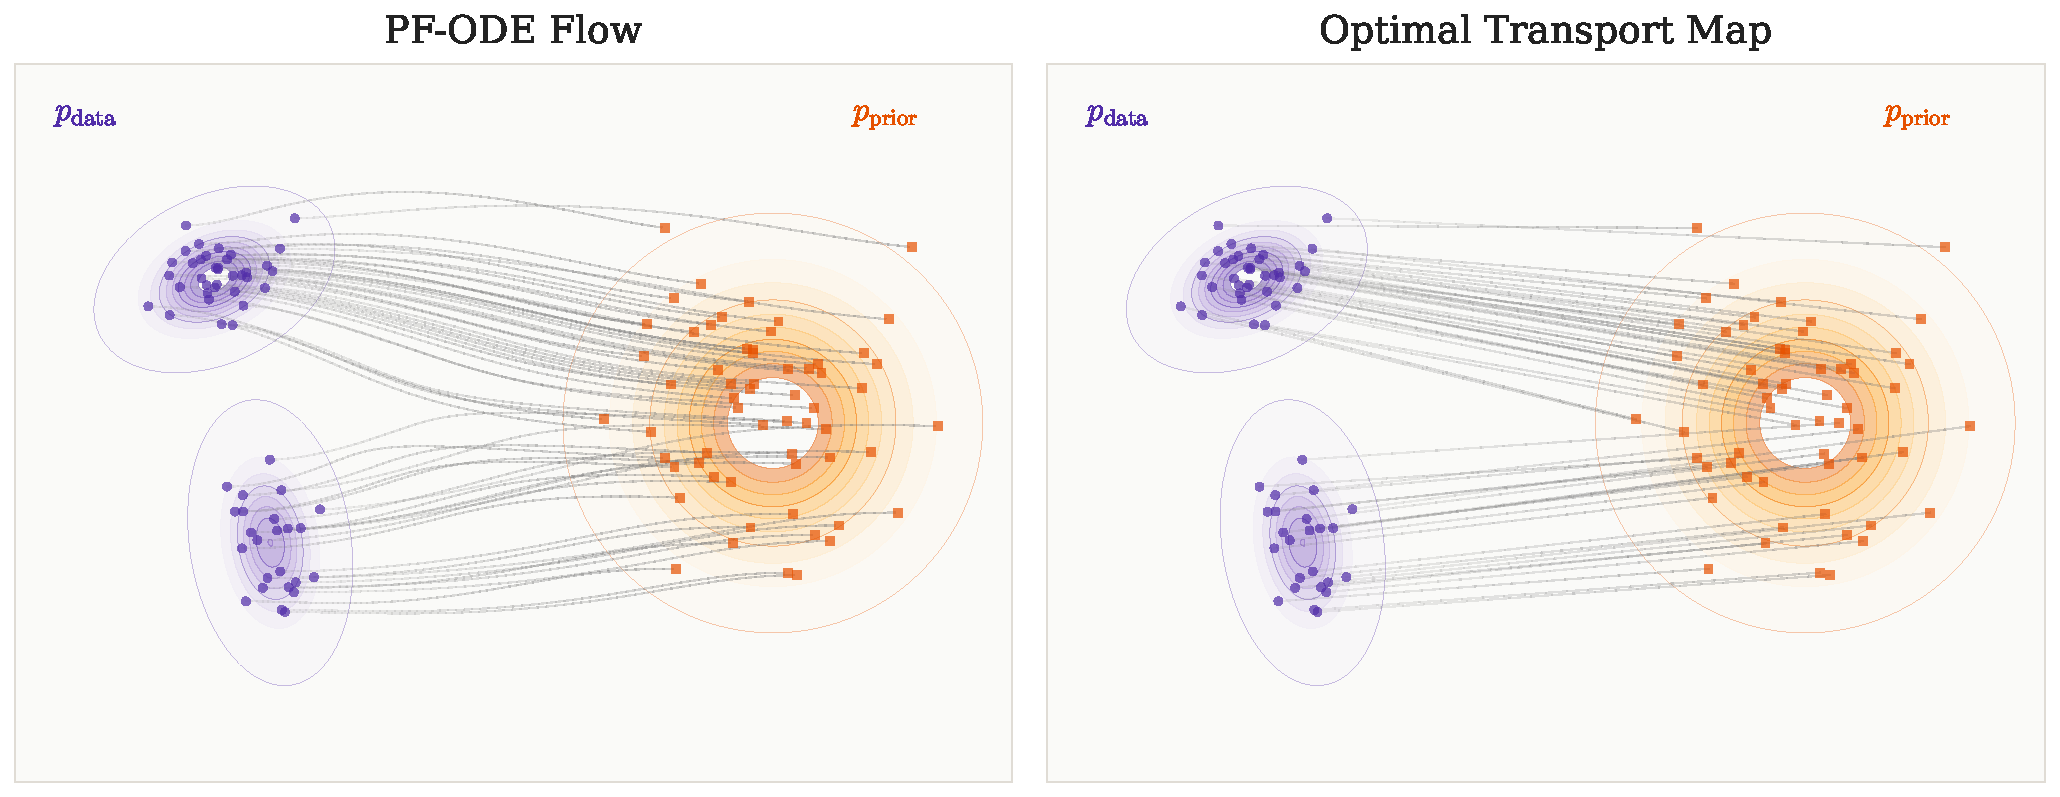
\includegraphics[width=\linewidth]{Images/PartB/pfode_vs_ot_2d.pdf}
    \caption{二维中从 $p_{\mathrm{data}}$ 到 $p_{\mathrm{prior}}$ 的 PF-ODE 流映射与真实 OT 映射的比较。
    右：二次代价 OT 映射，通过匈牙利算法精确计算。
    左：通过积分 PF-ODE 得到的 PF-ODE 流映射。两个映射明显不同，
    说明 PF-ODE 一般不能恢复最优传输映射。
    \figcredit{由作者在 AI 辅助编程下绘制。}}
    \label{fig:pfode-vs-ot-2d}
\end{figure}


\paragraph{设定。} 我们考虑 VP SDE，具体为 Ornstein–Uhlenbeck 过程，它将光滑初始密度 $p_0$ 演化为标准高斯 $\mathcal{N}(\bm{0}, \rmI)$：
\[
\diff \rvx(t) = -\rvx(t) \diff t + \sqrt{2} \diff \rvw(t), \quad \rvx(0) \sim p_0.
\]
相应的 PF-ODE 为
\[
\frac{\diff \mathbf{S}_t(\rvx)}{\diff t} = -\mathbf{S}_t(\rvx) - \nabla \log p_t(\mathbf{S}_t(\rvx)), \quad \mathbf{S}_0(\rvx) = \rvx.
\]
这里 $\mathbf{S}_t$ 表示将 $p_0$ 前推到边际 $p_t$ 的流映射：
\[
\left(\mathbf{S}_t\right) \# p_0 = p_t,
\quad\text{即}\quad
p_t(\rvy) = \int_{\mathbb{R}^D} \delta(\rvy - \mathbf{S}_t(\rvx))   p_0(\rvx) \diff \rvx.
\]
这些密度 $p_t$ 通过 Fokker-Planck 方程演化：
\[
\frac{\partial p_t}{\partial t} = \nabla \cdot (\rvx p_t) + \Delta p_t.
\]
这等价于具有如下速度场的连续性方程：
\[
\rvv_t(\rvx) = -\rvx - \nabla \log p_t(\rvx),
\]
其流由 $\mathbf{S}_t(\rvx)$ 给出。换言之，PF-ODE 可写为： 
\[
\frac{\diff \mathbf{S}_t(\rvx)}{\diff t} = \rvv_t\left(\mathbf{S}_t(\rvx)\right).
\]

当 $t \to \infty$ 时，该映射将初始分布传输到先验：
\[
\mathbf{S}_\infty \# p_0 = \mathcal{N}(\bm{0}, \rmI) =: p_{\text{prior}}.
\]
\paragraph{\citet{lavenant2022flow} 论证的目标。}

\citet{lavenant2022flow} 并不直接评估从 $p_0$ 到高斯的终端映射 $\mathbf{S}_\infty$ 是否最优。相反，他们构造一个特定的初始分布 $p_0$ 并考察整条 PF-ODE 轨迹。他们的关键观察是，最优性可能在流的某个点上失效。

他们考虑中间边际 $p_t = \mathbf{S}_t \# p_0$，并定义从 $p_{t_0}$ 到高斯的残差传输映射为
\[
\mathbf{T}_{t \to \infty} := \mathbf{S}_\infty \circ \mathbf{S}_{t}^{-1}, \quad \text{对所有 } t\geq 0.
\]
他们论证的核心是，对于精心选择的 $p_0$，存在一个时刻 $t_0 \geq 0$ 使得 $\mathbf{T}_{t_0 \to \infty}$ 不是从新的起始分布 $p_{t_0}$ 到 $\mathcal{N}(\bm{0}, \rmI)$ 的二次代价最优传输映射。

这一结果表明，PF-ODE 流一般并不产生最优传输映射，并且最优性这一性质对某些初始分布可能失效。

\paragraph{一些工具。} \citet{lavenant2022flow} 的论证关键依赖以下结果，即\emph{Brenier 定理}：
\begin{quote}
    \begin{theorem}[非正式的 Brenier 定理]\label{thm:brenier}
设 $\nu_1, \nu_2$ 为 $\mathbb{R}^D$ 上具有光滑密度的两个概率分布。一个光滑映射 $\rmT : \mathbb{R}^D \to \mathbb{R}^D$ 是从 $\nu_1$ 到 $\nu_2$（在二次代价下）的最优传输，当且仅当 $\rmT = \nabla u$，其中 $u$ 为某个凸函数。此时 $\mathrm{D} \rmT$ 对称且半正定，且 $u$ 满足 Monge–Ampère 方程：
\[
\det \mathrm{D}^2 u(\mathbf{x}) = \frac{\nu_1(\mathbf{x})}{\nu_2(\nabla u(\mathbf{x}))}.
\]
\end{theorem}
\end{quote}

证明还隐式地使用了如下事实，我们不再每次重复：\emph{一个映射是两个分布之间的最优传输，当且仅当其逆映射是反方向上的最优传输}。




\paragraph{证明梗概：PF-ODE 一般不是 OT 映射。} \citet{lavenant2022flow} 采用反证法：他们假设对每个 $t\ge0$，映射
\[
\mathbf{T}_t  =  \mathbf{S}_t \circ \mathbf{S}_\infty^{-1}
\]
是从 $\mathcal{N}(\bm{0},\rmI)$ 到 $p_t$ 的二次代价最优传输映射。




\subparagraph{第 1 步：Brenier 定理。}  由 Brenier 定理，从高斯出发的任何最优传输映射的雅可比必须对称且半正定。因此， 
\[
\mathrm{D} \mathbf{T}_t(\rvx) = \mathrm{D} \mathbf{S}_t(\mathbf{S}_\infty^{-1}(\rvx)) \mathrm{D} (\mathbf{S}_\infty^{-1})(\rvx)
\]
对所有 $t$ 和 $\rvx$ 必须对称。这里 $\mathrm{D} \mathbf{T}_t(\rvx)$ 表示关于 $\rvx$ 的全微分。
\subparagraph{第 2 步：对对称性条件关于时间求导。}  
关于时间求导：
\[
\frac{\partial}{\partial t} \mathrm{D}\mathbf{T}_t(\rvx)
= \left( \frac{\partial}{\partial t} \mathrm{D} \mathbf{S}_t \right)(\mathbf{S}_\infty^{-1}(\rvx)) \mathrm{D} (\mathbf{S}_\infty^{-1})(\rvx).
\]
鉴于对称性对所有 $t$ 成立，该导数也保持对称。

利用流 ODE（关于 $\rvx$ 求导），我们得到：
\[
\frac{\partial (\mathrm{D}\mathbf{S}_t)}{\partial t}
= \mathrm{D}\rvv_t(\mathbf{S}_t) \cdot \mathrm{D}\mathbf{S}_t
= \left( -\rmI - \mathrm{D}^2 \log p_t(\mathbf{S}_t) \right) \cdot \mathrm{D}\mathbf{S}_t.
\]
综合以上，我们看到
\[
\left( -\rmI - \mathrm{D}^2 \log p_t(\mathbf{S}_t) \right) \cdot\mathrm{D}\mathbf{S}_t \cdot \mathrm{D} (\mathbf{S}_\infty^{-1})
\]
对所有 $t\geq 0$ 对称。

在 $t = 0$ 处，我们有 $\mathbf{S}_0 = \rmI$ 且 $\mathrm{D}\mathbf{S}_0 = \rmI$，得到：
\[
\left( -\rmI - \mathrm{D}^2 \log p_0(\mathbf{S}_\infty^{-1}(\rvx)) \right) \cdot \mathrm{D} (\mathbf{S}_\infty^{-1})(\rvx) \quad \text{对称}.
\]

\subparagraph{第 3 步：交换性条件。}  由于假设 $\mathbf{T}_0 = \mathbf{S}_\infty^{-1}$ 是最优的，其雅可比 $D\mathbf{T}_0 = \mathrm{D}(\mathbf{S}_\infty^{-1})$ 对称。  此外，海森矩阵 $\mathrm{D}^2\log p_0$ 对称。  回顾两个对称矩阵相乘得到对称矩阵，当且仅当它们可交换。  因此，对所有 $\mathbf{x}\in\mathbb{R}^D$，
\[
\mathrm{D}^2\log p_0\bigl(\mathbf{S}_\infty^{-1}(\mathbf{x})\bigr)
\quad\text{必须与}\quad
\mathrm{D}(\mathbf{S}_\infty^{-1})(\mathbf{x})
\quad\text{可交换。}
\]
令 $\mathbf{y}=\mathbf{S}_\infty^{-1}(\mathbf{x})$ 得到等价条件：对所有 $\rvy\in\mathbb{R}^D$，
\[
\mathrm{D}^2\log p_0(\mathbf{y})
\quad\text{必须与}\quad
\mathrm{D}\mathbf{S}_\infty(\mathbf{y})
\quad\text{可交换。}
\]


现在，我们将这一条件转化为更可计算的形式。  
由于 $\mathbf{S}_\infty$ 在 $p_0$ 与 $\mathcal{N}(\bm{0},\rmI)$ 之间是最优的，Brenier 定理保证 $\mathbf{S}_\infty = \nabla u$，其中 $u$ 为某个凸函数。  由 Monge–Ampère 方程可得：
\[
\log p_0(\rvy) = \log \det(\mathrm{D}^2 u(\rvy)) - \frac{1}{2} \|\nabla u(\rvy)\|^2 + \text{Constant}.
\]
条件变为（其中 $\mathrm{D}\rmS_\infty = \mathrm{D}^2 u$）： 
\begin{mdframed}
\begin{align}\label{eq:necessary-ot}
\mathrm{D}^2 \left(\log \det \mathrm{D}^2 u - \frac{1}{2} \|\nabla u\|^2\right)
\quad\text{必须与}\quad
\mathrm{D}^2 u
\quad\text{可交换。}
\end{align}
\end{mdframed}
这给出了 $\mathbf{T}_t$ 为最优的一个必要条件。
\subparagraph{第 4 步：构造反例。} 让我们说明如何利用这一必要条件导出矛盾。

假设我们能构造一个凸函数 $u$ 使得  
\[
\mathrm{D}^2 \left( \log \det \mathrm{D}^2 u(\mathbf{x}) - \frac{1}{2} \lvert \nabla u(\mathbf{x}) \rvert^2 \right)
\]
不与 $\mathrm{D}^2 u(\mathbf{x})$ 对某个 $\mathbf{x} \in \mathbb{R}^D$ 可交换。  定义 $p_0 = (\nabla u)^{-1} \# \mathcal{N}(\bm{0}, \rmI)$，Brenier 定理蕴含 $\nabla u$ 是从 $p_0$ 到 $\mathcal{N}(\bm{0}, \rmI)$ 的最优传输。然而，\Cref{eq:necessary-ot} 中的条件失效，导致矛盾。因此，我们的目标是构造这样一个函数。 
考虑  
\[
u(\mathbf{x}) = \frac{1}{2} \|\mathbf{x}\|^2 + \varepsilon \phi(\mathbf{x}), \quad \text{对小的 } \varepsilon.
\]
则 $\mathrm{D}^2 u(\mathbf{0}) = \rmI + \varepsilon \mathrm{D}^2 \phi(\mathbf{0})$，且在 $\mathbf{x} = \mathbf{0}$ 处的可交换条件要求 $\mathrm{D}^2 \phi(\mathbf{0})$ 与 $\mathrm{D}^2 (\Delta \phi)(\mathbf{0})$ 可交换。 

例如，在 $\mathbb{R}^2$ 中，取  
\[
\phi(x_1, x_2) = x_1 x_2 + x_1^4
\]
便给出一个反例，其中海森矩阵 $\mathrm{D}^2 \log p_0$ 与雅可比 $\mathrm{D}^2 u$ 不可交换。

这一矛盾表明 $\mathbf{T}_t$ 不可能对所有 $t \geq 0$ 都最优。因此，存在某个 $t_0 \geq 0$ 使得映射 $\mathbf{T}_{t_0 \to \infty}$ 非最优。

\newpage 

\subsection{典型线性流与回流能否导出 OT 映射？}\label{subsec:ot-linear-reflow} 
我们已经看到 PF-ODE（尤其在前向核为 VP 型时）一般不是 OT 映射。现在一个自然的问题是：
\begin{question}
当将线性插值流 $(1-t)\rvx_0 + t \rvx_1$（其中 $\rvx_0\sim p_{\mathrm{src}}$、$\rvx_1\sim p_{\mathrm{tgt}}$）应用于独立耦合 $\pi(\rvx_0, \rvx_1) = p_{\mathrm{src}}(\rvx_0)p_{\mathrm{tgt}}(\rvx_1)$ 时，它能恢复 OT 映射吗？
\end{question}
问题的答案是否定的。
 
然而，将线性路径与给定耦合相结合，为真实 OT 代价提供了一个实用的上界。  在所有可能的路径中，线性插值提供了最紧的此类上界，正如我们在以下讨论中将看到的那样。


\paragraph{典型线性流与最优传输。}
聚焦于二次代价的最优传输，我们考虑 \Cref{eq:ot} 的等价形式，即 \Cref{eq:bb-ot} 中的 Benamou--Brenier 形式：
\begin{equation*}
    \mathcal{K}\left(p_{\mathrm{src}}, p_{\mathrm{tgt}}\right) :=  \min_{\substack{ (p_t, \rvv_t) \text{ s.t. }
        \partial_t p_t + \nabla \cdot (p_t \rvv_t) = 0, \\
        p_0 = p_{\mathrm{src}},\,\, p_1 = p_{\mathrm{tgt}}
    }}
    \int_0^1 \int_{\mathbb{R}^D} \|\rvv_t(\rvx)\|^2 p_t(\rvx) \diff\rvx \diff t.
\end{equation*}
不同于静态 Monge 形式（\Cref{eq: Monge's Formulation}），
其中计算最优映射需要求解 Monge--Amp\`ere
方程（\Cref{eq:monge-ampere}），Benamou--Brenier 问题在引入动量场
$\rvm_t := p_t \rvv_t$ 后允许一个凸重构。然而，将这一凸问题
在 $\mathbb{R}^D$ 的网格上离散化在高维下仍然不可处理。




虽然求解 Benamou-Brenier 形式一般不可行，但 \citet{liu2022rectified,lipman2024flow} 揭示其动能有一个实用的上界。这通过将搜索限制在更简单的\emph{条件流}族上来实现，其中每条路径由取自源分布与目标分布的某个耦合 $\pi_{0,1}$ 的固定端点 $(\rvx_0, \rvx_1)$ 定义。在这一\emph{条件流}族中，典型线性插值作为最优选择出现，如下面所形式化。

\proppp{通过条件流给出 OT 动能的上界}{ot-conditional-flow}{
设 $\pi_{0,1}$ 为 $p_{\mathrm{src}}$ 和 $p_{\mathrm{tgt}}$ 之间的任意耦合。
\begin{enumerate}
    \item[(1)] 动能以连接端点的任意条件流 $\bm{\Psi}_t(\rvx_0, \rvx_1)$ 的期望路径能量为上界：
    \begin{equation*}
        \mathcal{K}\left(p_{\mathrm{src}}, p_{\mathrm{tgt}}\right) \le \mathbb{E}_{(\rvx_0, \rvx_1) \sim \pi_{0,1}} \left[ \int_0^1 \|\bm{\Psi}'_t(\rvx_0, \rvx_1)\|^2 \diff t \right].
    \end{equation*}
    \item[(2)] 最小化右侧上界的唯一条件流 $\bm{\Psi}^*_t$ 是线性插值路径：
    \begin{equation*}
        \bm{\Psi}^*_t(\rvx_0, \rvx_1) = (1 - t) \rvx_0 + t \rvx_1.
    \end{equation*}
  代入这一最优路径得到最紧形式的上界：
    \begin{equation*}
        \mathcal{K}\left(p_{\mathrm{src}}, p_{\mathrm{tgt}}\right) \le \mathbb{E}_{(\rvx_0, \rvx_1) \sim \pi_{0,1}} \|\rvx_1 - \rvx_0\|^2.
    \end{equation*}
\end{enumerate}
}{证明依赖于 Jensen 不等式和条件期望的塔性质的直接应用，然后用 Euler-Lagrange 方程求解简化后的变分问题；完整论证参见 \citep{lipman2024flow} 的第 4.7 节。}

换言之，线性插值 $\bm{\Psi}^*_t$（即 Flow Matching 与 Rectified Flow 使用的前向核）对任意所选耦合 $\pi_{0,1}$，最小化了真实动能的一个上界。

我们强调，在此类条件流中的最优性并不保证在边际分布上的全局最优性。




\paragraph{回流与最优传输。} 
两个分布之间最朴素的传输方案，是使用简单的独立耦合以直线连接它们的样本。然而，这种方法明显不是最优的，因为问题不在于直线路径本身，而在于点的低效初始配对。

回流（Reflow）过程可能提供一种构造性的回应。它是一种专门为纠正这种配对而设计的迭代算法，并且关键是，每一步都保证代价非增 \citep{liu2022flow}。这一性质表明回流系统地将传输方案推向更优的配置，这自然地引出了关于其收敛性的核心问题。
\begin{question}
    如果我们迭代地应用 \texttt{Rectify} 算子会怎样？得到的传输方案序列能否收敛到最优方案，或者回流过程的不动点是否给出 OT 映射？
\end{question}
简短的答案在一般情况下是否定的。下面我们解释可能出什么问题。回顾一下，回流过程通过如下更新迭代地精炼 $p_{\mathrm{src}}$ 与 $p_{\mathrm{tgt}}$ 之间的耦合：
\[
\pi^{(k+1)} = \texttt{Rectify}(\pi^{(k)}),
\]
以乘积耦合 $\pi^{(0)} := p_{\mathrm{src}}(\rvx_0) p_{\mathrm{tgt}}(\rvx_1)$ 初始化。更确切地说，$\texttt{Rectify}$ 通过如下方式输出更新后的耦合 $\pi^{(k+1)}$：在每次迭代 $k = 0, 1, 2, \ldots$，通过如下方式学习一个速度场 $\rvv_t^{(k)}$：
\[
\rvv_t^{(k)} \in \argmin_{\rvu_t} \, \mathcal{L}(\rvu_t\big\vert\pi^{(k)}),
\]
其中 $\mathcal{L}(\rvu_t\big\vert\pi^{(k)})$ 是 \Cref{eq:reflow-loss} 中定义的损失（如 RF 或 FM 损失）。这里为记号简便，我们采用速度场的非参数形式，而非其他情形下使用的参数化形式 $\bm{\phi}$。
更新后的耦合由下式给出：
\[
\pi^{(k+1)}(\rvx_0, \rvx_1) := p_{\mathrm{src}}(\rvx_0)\, \delta\big(\rvx_1 - \bm{\Psi}_1^{(k)}(\rvx_0)\big),
\]
其中 $\bm{\Psi}_1^{(k)}$ 表示从初始条件 $\rvx_0$ 出发积分 $\rvv_t^{(k)}$ 在时间 $t=1$ 处得到的解映射。

在 \citep{liu2022flow} 中观察到，对于 $p_{\mathrm{src}}$ 与 $p_{\mathrm{tgt}}$ 之间的耦合 $\pi$，存在一个最小化回流损失的速度场 $\rvv_t$（即满足 $\mathcal{L}(\rvv_t |\pi) = 0$），这并不一定蕴含该传输是最优的。



受 Benamou–Brenier 框架（其中已知最优传输速度是某个势函数的梯度）启发，\citet{liu2022rectified} 提出了一个附加约束：速度场 $\rvv_t$ 应当是势场。相应地，\Cref{eq:reflow-loss} 中的目标被修改为将 $\rvv_t$ 限制在梯度向量场空间（也称为势流）中：
\begin{align}\label{eq:reflow-loss-gradient}
    \rvw_t^{(k)} \in \argmin_{\substack{\rvu_t:\, \rvu_t=\nabla\varphi \\ \text{对某个 }\varphi\colon\mathbb{R}^D\to\mathbb{R}}} \, \mathcal{L}(\rvu_t\big\vert\pi^{(k)}),
\end{align}
其余过程与 \texttt{Rectify} 中保持相同。
我们将这一相关算子记为 $\texttt{Rectify}_{\perp}$，强调其到无旋向量场的投影。

设 $\pi$ 为 $p_{\mathrm{src}}$ 与 $p_{\mathrm{tgt}}$ 之间的耦合。\citet{liu2022flow} 猜想如下刻画最优性的等价性：
\begin{enumerate}[label=(\textit{\roman*})]
  \item $\pi$ \textit{是最优传输耦合。}
  \item $\pi$ \textit{是势整流算子的不动点：}
  \[
    \pi = \texttt{Rectify}_{\perp}(\pi).
  \]
  \item \textit{存在一个梯度速度场 $\rvv_t = \nabla \varphi_t$ 使得整流损失为零：}
  \[
    \mathcal{L}(\rvv_t |\pi) = 0.
  \]
\end{enumerate}
然而，\citet{hertrich2025relation} 展示了两类反例：
\begin{enumerate}
  \item 当中间分布 $p_t$ 具有不连通支撑时，可以找到 $\texttt{Rectify}_{\perp}$ 的不动点，其回流损失为零且速度场为梯度场，但仍然无法产生最优耦合。
  \item 即使两个端点分布都是高斯分布，也存在损失任意小但偏离最优耦合任意大的耦合。
\end{enumerate}

因此，尽管整流流可能产生强大的生成模型，其作为最优传输求解器的可靠性仍然有限。这突显了生成建模与有原则的最优传输理论之间的重要差距，为二者交叉领域的进一步研究提供了契机。

最后，我们指出传输代价并不总是与下游性能相关；因此，计算精确的最优传输映射未必会带来更好的实际效果。尽管如此，最优传输的变体在科学与工程的许多问题中仍然具有基础性地位。扩散模型为探索这些挑战提供了一个强大的框架。

\newpage
\section{结束语}
在本章中，我们通过最优传输及其熵正则化变体的视角，重新审视了将一个
分布传输到另一个的经典问题。我们回顾了最优传输的静态
Monge--Kantorovich 形式与动态 Benamou--Brenier 形式，
其中传输由最小化动能代价的确定性流实现。随后我们讨论了熵正则化最优传输与
薛定谔桥（SB），它们用相对于参考过程最可能的受控扩散取代确定性传输。从
这一视角看，扩散模型在随机侧自然地接近 SB 的观点，
而其 PF-ODE 在 ODE 侧定义确定性
传输映射。然而，正如我们所强调的，PF-ODE
传输一般\emph{不是}二次代价最优传输
映射：它是众多确定性耦合之一，而非
Benamou--Brenier 作用量的最小化子。

这还突显了一个更基本的问题：在询问一个
传输是否最优之前，\emph{两个分布何时能完全由确定性映射连接？} 在许多设定下，存在性并非主要
困难。在温和的正则性假设下，常常能找到一个
可测映射 $\rmT$ 使得
$\rmT_\# p_{\mathrm{src}} = p_{\mathrm{tgt}}$。更困难的问题在于，
在一维以上，相对较少的经典构造既
显式又在实践中稳健。在一维中，单调
重排通过匹配分位数给出简单答案。在高维中，已知若干重要构造：Brenier 定理
（定理~\ref{thm:brenier}）在适当正则性下给出二次代价最优映射；Knothe--Rosenblatt
重排~\citep{rosenblatt1952remarks,knothe1957contributions}
由迭代的条件分布构造三角映射；而
Dacorogna--Moser 方法~\citep{dacorogna1990partial} 通过求解散度
方程的速度场构造光滑
微分同胚传输。每种方法都给出有原则的确定性传输途径，但
也都依赖于结构性假设或非平凡的分析
工具。

从这一视角看，基于扩散的流映射提供了一种有吸引力且
灵活的替代方案。扩散模型与流匹配方法不规定一个闭式传输
映射，而是学习一个随时间变化的
向量场，其诱导流将一个简单源分布推向
目标。这种学习到的映射不必与 Brenier
映射或任何其他经典的典型构造重合，且一般而言它
并不求解预定的最优传输问题。尽管如此，它
提供了一条实用且富有表达力的途径，用于高维下基于映射的采样，而那里
显式传输映射构造常常
不可用或难以计算。在这个意义上，扩散流最好
不被理解为经典传输理论的替代品，而是
现代学习到的传输机制，与最优
传输映射、三角重排以及基于 PDE 的构造
并列存在于确定性传输的更广阔图景之中。
\newpage
